\documentclass[]{elsarticle} %review=doublespace preprint=single 5p=2 column
%%% Begin My package additions %%%%%%%%%%%%%%%%%%%
\usepackage[hyphens]{url}

  \journal{Journal of Human Evolution} % Sets Journal name


\usepackage{lineno} % add
\providecommand{\tightlist}{%
  \setlength{\itemsep}{0pt}\setlength{\parskip}{0pt}}

\usepackage{graphicx}
\usepackage{booktabs} % book-quality tables
%%%%%%%%%%%%%%%% end my additions to header

\usepackage[T1]{fontenc}
\usepackage{lmodern}
\usepackage{amssymb,amsmath}
\usepackage{ifxetex,ifluatex}
\usepackage{fixltx2e} % provides \textsubscript
% use upquote if available, for straight quotes in verbatim environments
\IfFileExists{upquote.sty}{\usepackage{upquote}}{}
\ifnum 0\ifxetex 1\fi\ifluatex 1\fi=0 % if pdftex
  \usepackage[utf8]{inputenc}
\else % if luatex or xelatex
  \usepackage{fontspec}
  \ifxetex
    \usepackage{xltxtra,xunicode}
  \fi
  \defaultfontfeatures{Mapping=tex-text,Scale=MatchLowercase}
  \newcommand{\euro}{€}
\fi
% use microtype if available
\IfFileExists{microtype.sty}{\usepackage{microtype}}{}
\bibliographystyle{elsarticle-harv}
\usepackage{longtable}
\usepackage{graphicx}
% We will generate all images so they have a width \maxwidth. This means
% that they will get their normal width if they fit onto the page, but
% are scaled down if they would overflow the margins.
\makeatletter
\def\maxwidth{\ifdim\Gin@nat@width>\linewidth\linewidth
\else\Gin@nat@width\fi}
\makeatother
\let\Oldincludegraphics\includegraphics
\renewcommand{\includegraphics}[1]{\Oldincludegraphics[width=\maxwidth]{#1}}
\ifxetex
  \usepackage[setpagesize=false, % page size defined by xetex
              unicode=false, % unicode breaks when used with xetex
              xetex]{hyperref}
\else
  \usepackage[unicode=true]{hyperref}
\fi
\hypersetup{breaklinks=true,
            bookmarks=true,
            pdfauthor={},
            pdftitle={Ecological perspectives on technological diversity at Kanjera South},
            colorlinks=false,
            urlcolor=blue,
            linkcolor=magenta,
            pdfborder={0 0 0}}
\urlstyle{same}  % don't use monospace font for urls

\setcounter{secnumdepth}{0}
% Pandoc toggle for numbering sections (defaults to be off)
\setcounter{secnumdepth}{0}


% Pandoc header
\usepackage{setspace}\doublespacing



\begin{document}
\begin{frontmatter}

  \title{Ecological perspectives on technological diversity at Kanjera South}
    \author[Eberhard Karls University of Tübingen]{Jonathan S. Reeves\corref{1}}
   \ead{jonathan.reeves@uni-tuebingen.de} 
    \author[The George Washington University]{David R. Braun\corref{2}}
   \ead{David\_Braun@gwu.edu} 
    \author[Max Planck Institute for the Science of Human History]{Emma Finestone\corref{3}}
   \ead{cat@example.com} 
    \author[The Graduate Center, City University of New York]{Thomas Plummer\corref{4}}
   \ead{derek@example.com} 
      \address[Eberhard Karls University of Tübingen]{Eberhard Karls University of Tübingen}
    \address[The George Washington University]{The George Washington University}
    \address[Max Planck Institute for the Science of Human History]{Max Planck Institute for the Science of Human History}
    \address[The Graduate Center, City University of New York]{The Graduate Center, City University of New York}
      \cortext[1]{Corresponding Author}
  
  \begin{abstract}
  The aspects of hominin behavior responsible for Oldowan stone tool
  variation has been the focus of much debate. There is some consensus
  that Oldowan artifact variation arises from a combination of ecological
  and cultural factors. These factors are often examined independently of
  one another. The diversity of raw material types and technological
  strategies present at the site of Kanjera South provide an opportunity
  to examine the interacting effect of ecology and culture on Oldowan
  stone tool variation. Here we combine previous analyses of raw material
  properties, provenience, and technology with quantitative measures of
  core reduction intensity and tool utilization to examine the influence
  of both ecological and techno-cultural factors on stone tool variation
  at Kanjera South. The results of this analysis show that technological
  variation at a Kanjera South reflects a dynamic relationship between raw
  material properties, provenance, and hominin mobility. Cores produced on
  raw materials from distant sources are more reduced than locally sourced
  raw materials. Distant raw materials are generally more resistant to
  edge attrition compared to those available locally which may have
  incentivized their transport over long distances. Moreover, the
  variation in stone tool reduction is not constistent with neutral models
  of stone tool transport and discard. This suggests that the lithic
  assemblage at Kanjera South may reflect a structured land-use strategy
  that may relate to the resource rich nature of the Homa Penninsula. This
  pattern of stone tool utilization also has an impact on the
  technological strategies employed by Oldowan tool makers at Kanjera
  South. Cores produced on raw materials from distant sources also exhibit
  more complex core reduction strategies than locally acquired materials.
  While this pattern is partially due to the differences the quality of
  knappable stone, bifacial centripetal and multifacial core reduction
  strategies also arise due to the continuous transport and use of exotic
  raw materials. These results demonstrate that ecological factors such as
  raw material provenience and physical properties have strong impacts on
  reduction intensity and the technological strategies utilized by
  hominins. Yet, not all stone tool variation at Kanjera South can be
  explained by this relationship. These results suggest that Oldowan stone
  tool variation should not be examined from a strictly ecological or
  technological perspective, but rather within the context of its broader
  cultural-ecological system.
  \end{abstract}
  
 \end{frontmatter}

\doublespacing

\hypertarget{introduction}{%
\section{Introduction}\label{introduction}}

The Oldowan is relatively simplistic as it consists primarily of core
and flake tools (Leakey 1971). In contrast to earlier typological
approaches, experimental models by (Toth 1985) suggest that the Oldowan
is a simple core and flake industry whose primary goal is the removal of
flakes with sharp cutting edges. In spite of its superficial simplicity,
Oldowan stone tool variation is a vast resource of information regarding
Early Pleistocene hominin behavior. Technological analyses show that
Oldowan hominins had at least a basic understanding of the general
principles of flaking and selection of suitable tool stones for artifact
manufacture (Braun et al. 2019; D. R. Braun, Plummer, Ferraro, et al.
2009; Delagnes and Roche 2005; de la Torre 2004; Roche et al. 1999;
Semaw 2000; Stout et al. 2005). In addition, Oldowan hominins also
transported stone tools various distance to the places where they are
used and discarded (Blumenschine and Peters 1998; D. R. Braun,
Ditchfield, et al. 2008; Harmand 2009; Hay 1976; Isaac 1984; Potts 1991;
Toth 1985). Despite early suggestions that the Oldowan was a largely
expedient tool kit (Chavaillon 1970), it may reflect a more nuanced
technical system, where raw material is acquired, transported, utilized,
maintained and eventually discarded (Isaac 1984).

A major difficulty in the study of Oldowan hominin behavior is linking
variation in artifacts to individual influences on behavior (Gallotti
2018; Roche, Blumenschine, and Shea 2009). While socio-cognitive
approaches only require examining technological strategies present in
the artifacts themselves, ecological analyses require integrated
ecological and functional data sets. Demonstrating the influence of
ecological parameters on stone tool use requires establishing spatial
relationships between measures of stone tool utilization and landscape
features such as raw material sources and paleogeographic settings
(Blumenschine and Peters 1998; Blumenschine et al. 2008; Blumenschine,
Stanistreet, and Masao 2012; @ D. R. Braun, Rogers, et al. 2008; D. R.
Braun, Plummer, Ditchfield, et al. 2009; Isaac and Isaac 1997; Rogers
1997). While previous work on this topic has demonstrated the influence
of raw material access on Oldowan assemblages (Blumenschine et al.
2008), little work has been done demonstrating its direct influence on
technological variation in the Oldowan. The site of Kanjera South
provides an opportunity to do so. Extensive research on the
technological context has characterized not only the technological
strategies employed by hominins, at this site, but also the landscape
context of the site (Behrensmeyer et al. 1995; D. R. Braun, Ditchfield,
et al. 2008; D. R. Braun, Plummer, Ditchfield, et al. 2009; D. R. Braun,
Plummer, Ferraro, et al. 2009; Ditchfield et al. 2018; Bishop et al.
2006; Kent 1942; Lemorini et al. 2014, 2019; Oliver et al. 2019;
Plummer, Bishop, et al. 2009; Plummer et al. 2001, 1999; Plummer and
Bishop 2016). Here we present an integrated approach that examines
Oldowan lithic technology from an ecological context. The results of
this study contribute to the exploration of ecological and
socio-cultural influences on Oldowan artifact variation.

\hypertarget{background}{%
\section{Background}\label{background}}

Given the dynamic system that Oldowan tools ultimately reflect, it is
argued that stone tool variation is influenced by function, ecology,
culture and cognition (Gallotti 2018; Isaac 1984; Plummer, Bishop, et
al. 2009; Toth and Schick 2006) (Figure \ref{variation}). Understanding
the role of function in shaping Oldowan stone tool variation is
constrained. The uses of Oldowan tools beyond evidence of cutting, and
flake production is not well known. A small number of use-wear studies
are beginning to shed light on the diversity of functions that Oldowan
flakes were used for (Keeley and Toth 1981; Lemorini et al. 2014, 2019).
The impact of these functions on Oldowan stone tool variation remains
unclear. As a result, Oldowan studies have focused primarily on drawing
behavioral inferences from explorations of hominin ecology, culture and
cognition derived from the morphological variation in stone tools.
However, these various aspects of hominin life-ways are seldom studied
in tandem.

\begin{figure}
\centering
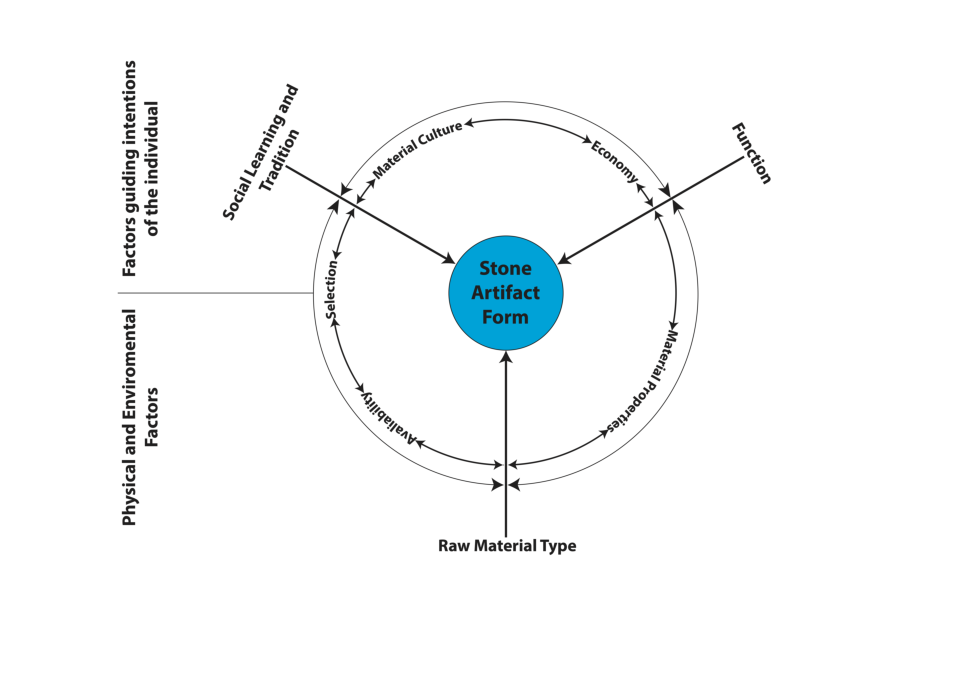
\includegraphics{Reeves_Braun_et_al_2020_Kanjera_South_JHE_files/figure-latex/unnamed-chunk-1-1.pdf}
\caption{A diagram of factors that contribute to stone tool variation.
Adopted from Isaac (1984). \label{variation}}
\end{figure}

The ecological approach views tools as an extra-somatic mechanism for
solving environmental problems (Binford 2001). This approach was
originally championed by the work of Glynn Isaac, John Desmond Clark,
and their students (Clark 1975; Harris 1978; Isaac and Isaac 1997; Shick
1987; Toth 1987, 1982). In this perspective technology is considered to
be a dynamic process that is adapted to the temporal and spatial
distribution of resources (Bamforth 1990; Isaac and Harris 1976; Isaac
1981; Ludwig and Harris 1998; Nelson 1991; Peters and Blumenschine 1995;
Rogers, Harris, and Feibel 1994; Toth 1985). In essence this approach
investigates artifacts as dynamic objects that are a part of the hominin
foraging system. One component of this approach is the concept that
artifacts reflect movement of stone resources across landscapes often
referred to as the ``the flow of stone'' model (Isaac 1984). Some
artifacts are produced and discarded whereas others are transported away
from the site. Understanding how this flow of stone through structured
landscapes produces inter-site assemblage variability provides insight
into the ecology and foraging strategies of early hominins
(Blumenschine, Stanistreet, and Masao 2012). As a result, a variety of
models have been proposed and debated for how assemblage composition,
lithic attributes and artifact density reflect land-use patterns at
multiple spatial scales (Binford 1976; Foley 1981a, 1981b; Isaac 1983,
1981; Isaac and Harris 1976; Shick 1987; Toth 1987). Ecologically
oriented research often measures aspects of stone tool variation in
relation to measures of tool utilization and transport. Quantitative or
ordinal variables such as mass, length, proportion of cortex, and flake
scar density are often compared alongside landscape variables such as
distance to raw material source and paleogeographic context (Andrefsky
2009, 2008; Blumenschine, Stanistreet, and Masao 2012; Bunn et al. 1980;
Davies, Holdaway, and Fanning 2018; Douglass 2010; Holdaway, Stern, and
Chauhan 2004; Brantingham 1998; Kuhn, Raichlen, and Clark 2016; Toth
1987). Examples of this type of approach includes studies of artifact
variation throughout the Okote Member of the Koobi Fora Formation.
Paleogeographic context appears to influence the transport patterns and
reduction intensity of these artifacts when they are discarded (@ D. R.
Braun, Rogers, et al. 2008; Rogers, Harris, and Feibel 1994; Rogers
1997; Stern, Porch, and Mcdougall 2002). At Olduvai, quartz artifacts
vary in size and abundance according to their distance from a large
outcrop of quartz called Naibor Soit (Blumenschine et al. 2008).Measures
of cortex and core reduction have shed light on the dynamic input-output
system under which Oldowan lithic assemblages form (Bunn et al. 1980;
Rogers 1997; Toth 1987; @ D. R. Braun, Rogers, et al. 2008).

An alternative approach to the ecological focus, is one where the
actions and thoughts associated with stone tool production are
highlighted (Sellet 1993). This is sometimes referred to as the
technological approach (Soressi and Geneste 2011). From this
perspective, the variation seen in all technology stems from socially
mediated images and thoughts (Inizan et al. 1999). The various
combinations of ways to flake, shape or retouch stone are argued to
reflect the different knapping strategies that characterize the skills
of a group or individual (Delagnes and Roche 2005). From this
perspective stone tools reflect the cognitive capacity and the technical
competence of Oldowan tool makers (Roche, Blumenschine, and Shea 2009;
Schick and Toth 1994; Stout et al. 2015; Stout and Chaminade 2009; Toth
and Schick 2018). In particular, certain components of the artifact
production process (e.g.~complex series of nested goals) appear to
require specific cognitive traits (Wynn and Coolidge 2016). Oldowan
variation is interpreted as differences in skills, cultural traditions,
or even different taxa (Delagnes and Roche 2005; Roche et al. 1999,
2018; Roche, Blumenschine, and Shea 2009; Stout et al. 2010).
Technological analyses have been instrumental in revealing the rules
that govern stone artifacts production. Analysis of lithic assemblages
from West Turkana in Kenya show that hominins had already mastered flake
removal and how to maintain and exploit pre-existing platforms (Delagnes
and Roche 2005).

Moreover, differences in the arrangement of flake scars, refit
sequences, the frequency of knapping accidents are used to infer
different production strategies from Oldowan lithic assemblages.
Differences in the inferred skill of toolmakers at Lokalelei 1 and 2c
are so striking that the author suggested that the differences arise
from 2 different social groups or possibly different species of hominins
(Delagnes and Roche 2005). At Gona, differences in the proportion of
reduction strategies between sites have been argued to reflect cultural
traditions of specific groups (Stout et al. 2010, 2019). At a broader
scale, some researchers have argued that the variation in the Oldowan is
similar to the regional variation in the observed in chimpanzee cultures
(Barham and Mitchell 2008; Whiten et al. 1999; Whiten, Schick, and Toth
2009). The social context within this variation is interpreted to
reflect potentially different social learning mechanisms in the
archaeological record (Morgan et al. 2015; Stout et al. 2019).

The vast majority of research on Oldowan artifacts can be identified as
falling into one the previously described categories (i.e.~either
ecologically focused or socially mediated). The singular focus of most
Oldowan research on either ecological or technological questions has an
impact on the current status of Oldowan research. The manner in which
the Oldowan is described, and the methods used to describe it, depend
heavily on the theoretical position of the analyst (la de Torre and Mora
2009). In a way, this is problematic because as figure \ref{variation}
demonstrates, the factors that contribute to stone tool variability are
not mutually exclusive and likely interact with one another For example,
the strategy used to reduce a core will affect the proportion of
different Toth types produced (Stout et al. 2019, 2010). This will also
likely influence how cortex is distributed across a landscape (Toth
1987). Therefore in the absence of a more integrated approach,
differences in the representation of flake types (i.e.~Toth Types)
between two sites could be interpreted as varied foraging techniques
when in reality they result from different tool reduction strategies (or
possibly a combination of both). Therefore, in this example, reduction
strategy and measurements of cortex must both be considered before
discussing the aspects of behavior reflected in a given assemblage. In
other words, without considering the broader ecological context of the
Oldowan it may be impossible to disentangle technical competence of
Oldowan knapppers from technological variability (or \emph{vice versa}).

Moreover, studies have demonstrated the presence of a distance - decay
relationships between the location of tool-stone sources and stone tool
discard in the Oldowan (Blumenschine et al. 2008; @ D. R. Braun, Rogers,
et al. 2008; Toth 1985). However, these patterns are often described in
terms of reduction intensity, size of flakes and cores, or the
representation of cortex. Oldowan cores that are more reduced often
involve greater levels of core rotation (Toth 1982). It is possible that
differences in technological strategies may sometimes arise due to raw
material abundance. Moreover, it may be that Oldowan stone tool
variation may be the result of a complex interaction between social
mechanisms of information transfer and ecological context. Understanding
the significance of Oldowan variability requires an integrated approach
which considers the context of tool use as well as the context of
availability of resources.The assemblage of Oldowan artifacts from
Kanjera South provide the opportunity to understand an artifact record
within the context of raw material availability and technological
variability (Plummer and Bishop 2016).

\hypertarget{background-to-kanjera-south}{%
\section{Background to Kanjera
South}\label{background-to-kanjera-south}}

\begin{figure}
\centering
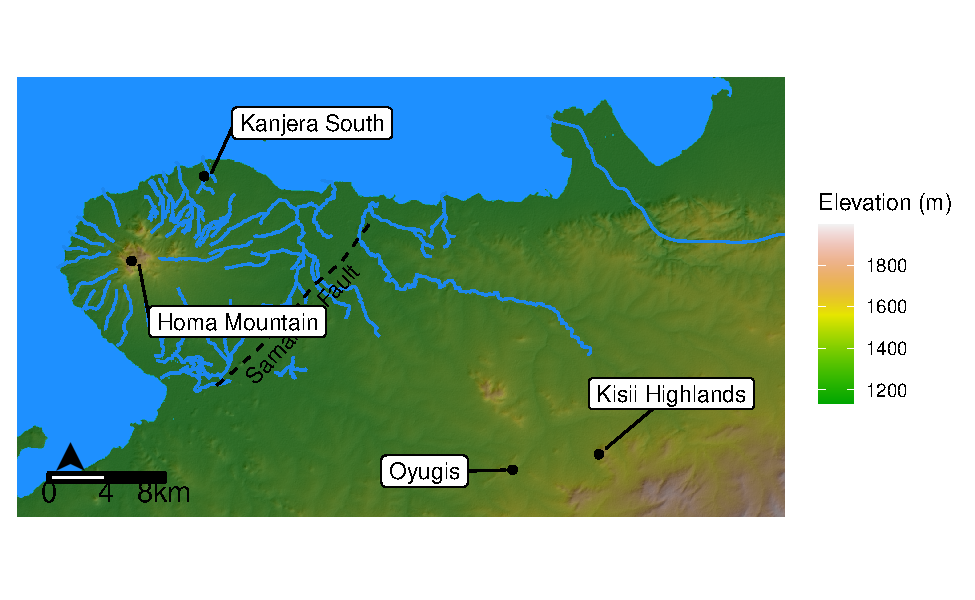
\includegraphics{Reeves_Braun_et_al_2020_Kanjera_South_JHE_files/figure-latex/unnamed-chunk-2-1.pdf}
\caption{A map of the Homa Peninsula. Kanjera South is situated to the
East of Homa Mountain. The Homa Mountain carbonatite center is the
primary source of the local raw materials including Homa limestone
(HLi), Homa Phonolite (HPh), and Fenetized nyanzian rocks (FNy). The
Kisii Highlands, where the distant or exotic raw materials originate are
situated farther to the east. These include Bukoban andesite (BBa),
Bukoban felsite (BFe), Bukoban quartzite (BQu), Nyanzian rhyolite (NyR),
and Oygus granite (OGr) \label{map}}
\end{figure}

The site of Kanjera South is situated on the northern side of the Homa
Peninsula on the edges of the Nyanza Rift near the shores of Lake
Victoria (Plummer, Ditchfield, et al. 2009; Plummer et al. 1999). The
archaeological site is in an amphitheater of sediment that has been
exposed by the Kanjera River that is draining off the Homa Mountain
carbonatite complex (digure: \textbackslash{}ref\{map\}). This volcanic
edifice dominates the sedimentary processes and basement geology of the
region (LeBas 1970). The site of Kanjera South was excavated from a 3
meter stacked sequence of clays and silts that record extensive hominin
behavior in the form of stone artifacts and bones with surface
modifications that are indicative of the butchery of meat and
acquisition of marrow (D. R. Braun, Plummer, Ditchfield, et al. 2009;
Plummer, Ditchfield, et al. 2009). Extensive excavation has recovered
over 3000 fossils and similar numbers of stone artifacts (Plummer,
Bishop, et al. 2009). The stratigraphy at Kanjera South is made up of
approximately 30 m of fluvial, colluvial and lacustrine sediments
(Ditchfield et al. 2018). This stratigraphic sequence is well dated to
\textasciitilde{}2. Ma using a combination of paleomagnetic and
biochronological markers. These sediments are formally assigned to the
Southern Member of the Kanjera Fm (Behrensmeyer et al. 1995; Plummer et
al. 1999). There are five beds at Kanjera South (from oldest to youngest
KS-1 to KS-5) with artifacts and fossils concentrated in the sands and
silts of upper KS-1 to KS-3 (Ditchfield et al. 2018). Lithics and
fossils are thought to have been predominantly accumulated by hominins
except for those found within thin, discontinuous conglomerates which
represent brief intervals of higher energy water flow (Ditchfield et al.
2018; Ferraro et al. 2013).

The lithic assemblage recovered from exacavations at Kanjera South
represents one of the largest single accumulations of Oldowan artifacts
in association with modified fossil bone (Plummer 2004). The largest
site (169 m\textsuperscript{2}) yielding the bulk of the archaeological
finds was Excavation 1. The frequencies of different bovids in these
beds indicates that the Kanjera South landscape, unlike the setting of
most of the Oldowan sites, was dominated by a grasslands as opposed to
trees (Plummer, Ditchfield, et al. 2009). This is further supported by
the stable isotope analysis of pedogenic carbonates and tooth enamel
indicating a relatively high proportion of plants that use a C4
photosynthetic pathway. The fossils associated with the stone artifacts
at Kanjera South exhibit substantial evidence of hominin involvement in
the accumulation of materials (Ferraro et al. 2013). Evidence from bone
surface modifications as well as the proportions of bones modified are
similar to patterns seen in ``hominin first'' experimental datasets for
small mammals, while larger mammals show more mixed access (Ferraro et
al. 2013). The totality of the zooarchaeological evidence at Kanjera
strongly implicates a scenario where hominins had early access to small
carcasses. Evidence from mortality profile data also supports the
inference that hominins may have been able to access smaller carcasses
prior to carnivores and that larger carcasses were at times scavenged
(Oliver et al. 2019).

The stone artifacts from Kanjera South reflect a wide diversity of
technological adaptations (D. R. Braun, Plummer, Ditchfield, et al.
2009). The high diversity of the local geology on the Homa Peninsula
provided a wide choice of different raw material types that hominins
could incorporate into their toolkit. There are 16 formally described
raw material types with many additional types that only appear in small
quantities within the assemblage (D. R. Braun, Plummer, Ditchfield, et
al. 2009). A detailed provenance study of the rock types used to make
stone artifacts at Kanjera documented two features that distinguish the
Kanjera South assemblage from many other Oldowan assemblages. The first
is the presence of transport to Kanjera South from conglomerates that
are at least 10 km away from the site (D. R. Braun, Ditchfield, et al.
2008). The second is the systematic selection of rocks that have
specific mechanical properties (D. R. Braun, Plummer, Ferraro, et al.
2009). Hominins selected rocks that fracture consistently and also had
edges that resisted wear. The selection of certain rock types exceeds
that which is seen in other Oldowan assemblages. Furthermore the
intensity of selective behaviors seems to parallel rock properties.
These differences in rock properties are reflected in the flaking
technology. Unidirectional and multidirectional flaking patterns feature
prominently in this assemblage. However, the flaking patterns track raw
materials differences and there appears to be a concerted effort to
extend the use life of cores in some raw materials by increasing the
length of flaking sequences in some raw materials. These different
technological strategies applied to different raw materials results in a
high diversity of core reduction strategies in the Kanjera South
Assemblage (D. R. Braun, Plummer, Ditchfield, et al. 2009).

In addition to information regarding the transport and selection of
certain raw materials, detailed studies of the micro-wear on the stone
artifacts from Kanjera provide insights into artifact use (Lemorini et
al. 2014, 2019). Usewear evidence suggests that the tool used by hominin
at Kanjera were used for a variety of different activities. Most of
these actions involve cutting, and the different raw materials appear to
be used on different substrates. Usewear studies also suggests that some
of the stone tools were used for modifying wood. This suggests that
hominins were using stone artifacts to fashion other wooden tools
(Lemorini et al. 2019). Combined with the transport information, the sum
of the information about stone artifacts at Kanjera South suggests that
stone artifacts represented a significant component of the extractive
foraging adaptation of Oldowan hominins.

\hypertarget{methods}{%
\section{Methods}\label{methods}}

Oldowan tools undergo a series of transformations, through the removal
of flakes, from the time they are acquired until they are ultimately
discarded (Andrefsky 2009). As reviewed above, the flake removal process
relates to a diversity of social and economic factors surrounding tool
use and production. Here we explore the interaction of these factors on
stone tool variability. As such, this study combines the pre-existing
knowledge of stone tool production regarding, raw material properties,
provenience and technology at Kanjera South with newly applied measures
of stone tool utilization. This provides a novel means to understand
Oldowan stone tool production from a multifaceted point of view in which
the relationships between stone tool utilization, landscape-scale raw
material constraints, and stone tool production strategies can be
investigated.

\begin{longtable}[]{@{}cccc@{}}
\caption{A list of rock types included in this analysis}\tabularnewline
\toprule
Raw.Material & Abreviation & Origin & Provenance\tabularnewline
\midrule
\endfirsthead
\toprule
Raw.Material & Abreviation & Origin & Provenance\tabularnewline
\midrule
\endhead
Fenetized nyanzian & FNy & Homa Mountain & Local\tabularnewline
Homa limestone & HLi & Homa Mountain & Local\tabularnewline
Homa phonolite & HPh & Homa Mountain & Local\tabularnewline
Bukoban andesite & BBa & Kisii Highlands & Exotic\tabularnewline
Bukoban felsite & Bfe & Kisii Highlands & Exotic\tabularnewline
Bukoban quartzite & Bqu & Kisii Highlands & Exotic\tabularnewline
Nyanzian rhyolite & NyR & Kisii Highlands & Exotic\tabularnewline
Oygus granite & Ogr & Oygus & Exotic\tabularnewline
\bottomrule
\end{longtable}

We characterize the technology of stone tools produced on both distant
and local materials at Kanjera South (Table 1) through the study of the
core and complete flake assemblages (i.e.~our analysis at this time does
not incorporate angular fragments). Tool utilization for cores was
measured in terms of reduction intensity. We estimate the proportion of
mass lost prior to its discard following the methods outlined in
(Douglass et al. 2017). In addition, tool utilization is also examined
by estimating the relative proportion of flakes in the Kanjera South
assemblage that derive from early or later parts of the reduction
sequence. We identify the sequence order that flakes were removed from
their cores by using previously published models that use quantitative
measures of flakes to predict their placement in a reduction sequence
(D. R. Braun, Tactikos, et al. 2008). Flake sequence refers to the order
that flake was removed from the core. Flake sequence data provides an
independent measure of tool utilization that could be compared to the
estimates of core reduction. Additionally, it also provides a way to
examine the amount of flake production that occurred at Kanjera South.
If cores were transported directly to Kanjera South and reduced, then
the early flake sequences (i.e.~the first flakes off the core) would be
present in the assemblage. However, if early stage flakes are not
present in the assemblage then it can be inferred that cores were
utilized elsewhere prior to their transport to and discard at Kanjera
South. Measures of core reduction intensity are analyzed along-side
technological strategies (e.g.~bidirectional) utilized in core
reduction. Furthermore, core reduction and flake sequence values can
also be examined according to raw material type. This provides a means
to examine the impact of raw material properties and provenience on core
reduction and technology. The integration of these multiple lines of
evidence allows us to place stone tool variability at Kanjera south
within the broader technological system in which it took place.

\hypertarget{characterizing-stone-tool-utilization.}{%
\subsection{Characterizing Stone Tool
Utilization.}\label{characterizing-stone-tool-utilization.}}

Tool utilization has been extensively researched in lithic analysis (see
Andfresky 2009 for overview). Most studies of tool utilization focus on
the degree of artifact reduction as a proxy for the use-life of an
artifact (although these things are related but they are not the same;
Shott (1996)). Reduction intensity can be calculated for a variety of
artifact types (Dibble 1995). Currently several methods exist for
estimating the extent of core reduction. The majority of these methods
rely on establishing linear relationships between core attributes and
the amount of mass lost during artifact production to predict mass
removed from a core (Clarkson 2013; Douglass et al. 2017). This study
uses the methods outlined in Douglass et al. (2017) to estimate core
reduction intensity as the proportion of mass lost.The predictive model
developed by Douglass et al. (2017) incorporates a series of core
attributes beyond simply surface area and total number of flake scars.
This model considers, the number of flake scars, exploitation surfaces,
the number of exploitation surface convergences, the proportion of
cortex, and average platform angle to estimate core reduction intensity.

The \emph{number of flake scars} intuitively refers to the number of
previous flake removals present on the core. The \emph{number of
exploitation surfaces} refers to the number of areas of the core where
flakes were removed along a similar axis. This variable is related to
core rotation which is argued to increase as core reduction increases
(e.g.~Delagnes and Roche 2005). The \emph{number of exploitation surface
convergences} documents the number of times different exploitation
surfaces intersect with each other. Throughout reduction exploitation
surfaces with different flaking axes tend to converge (Braun 2005,
Douglass et al 2017). The proportion of cortex has an intuitive
relationship with core reduction intensity. That is, the total
proportion of the core that possesses cortical surface area will
diminish during reduction. \emph{Average platform angle}, measured in
degrees, refers to the mean angle between striking surfaces. Various
experimental replication studies show that, as this angle approaches
90°, it becomes increasingly difficult to detach a flake (Cotterell,
Kamminga, and Dickson 1985). Therefore, as a core approaches exhaustion,
the platform angles on the core are likely to approach 90° (Douglass et
al. 2017). Specifically, the method by Douglass et al. (2017) utilizes a
generalized linear mixed model to examine the effects of predictor
variables on core reduction intensity and ultimately predict the
percentage of mass lost from a core. The added benefit of this model is
that it is directly applicable to the materials analyzed in here, as it
is was developed in validated on experimental material and a subset of
archaeological material from Kanjera South (D. R. Braun, Tactikos, et
al. 2008). These details are discussed in Douglass et al. (2017).

\hypertarget{flake-sequence-estimates}{%
\subsection{Flake Sequence Estimates}\label{flake-sequence-estimates}}

Flake sequence is a common analytical method in American archaeology
(Andrefsky 2009; Bamforth 1986) but is also applied to Early Stone Age
assemblages in various forms (D. R. Braun, Tactikos, et al. 2008; de la
Torre Ignacio 2011; Stout et al. 2010; Toth 1985). In the Early Stone
Age, flake sequences are most commonly characterized using Toth types,
which classifies flakes into six different stages depending on the
presence of cortex on a flake's platform and dorsal surface (Toth 1985).
Here we follow D. R. Braun, Tactikos, et al. (2008), using a
multi-linear model to estimate flake sequence values. This methodology
is specifically focused on understanding the approximate location of a
flake within a reduction sequence. Unlike Toth's flake types, which is
focused on relative sequence information, the multi-linear model allows
for an absolute placement of a flake within a reduction set (within a
prescribed error). The multiple linear regression uses flake length,
width, number of platform facets, number of flake scars, and the number
of flake scar directions; specific details for each measurement are
clearly outlined in D. R. Braun, Tactikos, et al. (2008) (page 2156,
figure 3). Before the sequence number can be estimated, the number of
flake scars and amount of dorsal cortex must be divided by the log of
the surface area of the flake (D. R. Braun, Tactikos, et al. 2008).
These variables are then used by the predictive model to estimate the
flake sequence number. Flake sequence estimates have a maximum error
between +/- 8 sequences. However, an application of the method to
refitting sequences from the Koobi Fora formation showed it always
places flakes in their relative order(D. R. Braun, Tactikos, et al.
2008). Therefore, while information derived from individual flake
sequence estimates may be coarse-grained, it remains useful for
assemblage scale comparisons.

\hypertarget{edge-to-mass-ratios}{%
\subsection{Edge to mass ratios}\label{edge-to-mass-ratios}}

Measurements of tool use are often associated with enumerating the
details of the reduction of artifacts (Dibble 1995; Eren and Sampson
2009). This is largely because of the reductive nature of stone
technology (i.e.~the process of producing stone tools always produces a
smaller byproduct). However, some have also reviewed the general
efficiency of this flaking process (Braun and Harris 2003; Brantingham
and Kuhn 2001; Eren, Greenspan, and Sampson 2008; Muller and Clarkson
2016). Unfortunately, the study of efficiency in artifact production is
not well standardized. There are some studies that investigate the
overall efficiency of specific knapping strategies (Brantingham and Kuhn
2001; Eren et al.~2008). Others review efficiency as it pertains to
individual flaking events within an overall technological framework
(Braun and Harris 2003). Identifying the mechanisms that result in
highly efficient tool forms is not well understood (Lin et al. 2013;
Dogandži\a'c, Braun, and McPherron 2015). Yet it is clear that there is
variation in how efficient some technologies are (even though the metric
for identifying efficiency is debated; Eren et al.~2008). Assuming that
most stone tools are produced to create sharp edges, one possible
measure is estimating the amount of sharp edge produced per given unit
of mass. Technologies that produced a higher amount of edge per volume
of material can be considered more efficient (Braun and Harris 2003).
Here we use a measure of edge that is based on tracing the edge of whole
flakes (Braun and Harris 2003; Isaac and Isaac 1997). To calculate
efficiency this edge estimate is divided by the logarithmic
transformation of mass. The reason for this transformation is that mass
increases in three dimensions (i.e.~volumetrically) and the edge of a
flake increases in two dimensions. The logarithmic transformation of
mass prevents distortions of this ratio that are the result of general
size parameters. For example, very small flakes have relatively high
edge for a given amount of mass, but this is not always the most
efficient way to produce the greatest amount of edge relative to volume
(e.g.~see discussions on this topic in Kuhn 1991). Flakes that have high
amounts of edged relative to their mass tend to be relatively thin
flakes, and there is the possibility that the efficiency of these tools
is limited by their capabilities to complete certain tasks (e.g.~tacks
that require intensive use of edges such as hide scraping may not be
feasible with relatively thin flakes). Here we calculate the edge to
mass ratio of flakes within raw material categories. We then aggregate
this measure across raw materials types to assess the overall efficiency
of a given raw material. These aggregate measures are likely more
reflective of the generalized pattern of efficiency in tool production
over time at the Kanjera South locality.

\hypertarget{results}{%
\section{Results}\label{results}}

\hypertarget{core-utilization}{%
\subsection{Core Utilization}\label{core-utilization}}

Core reduction intensity estimates reveal that there is a wide range of
variation in the amount of mass that was removed from the cores at
Kanjera South. Some cores were minimally utilized whereas others were
reduced as much as 95\% of their original mass. There is also a
significant relationship between core reduction intensity and raw
material type (Kruskal-Wallis, p = \textless{} .0001). This pattern
appears to be driven by raw material provenance. Cores produced on raw
material types that originate from more distant sources (BBA, BFE, BQU,
NYR, and OGR) are on average more substantially reduced than those that
occur locally (FNy, HPh, HLi) (Kruskal-Wallis, p \textless{} .0001,
Figure: \ref{core_redux_rm}).

\begin{figure}
\centering
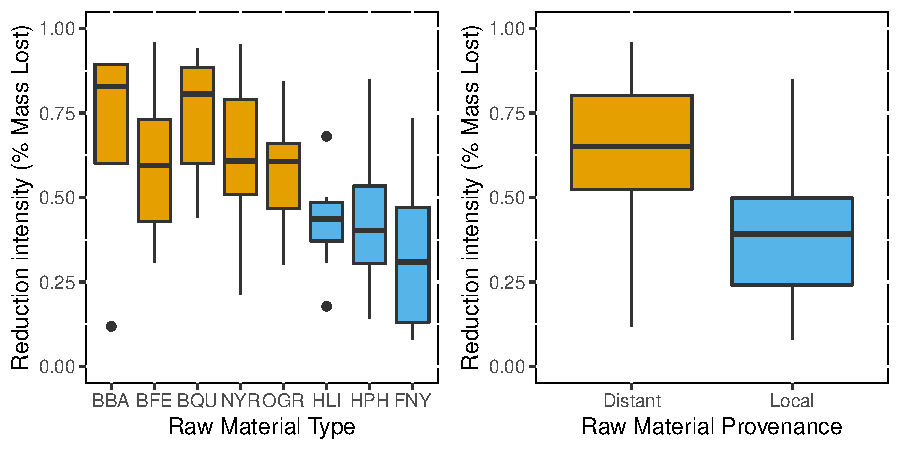
\includegraphics{Reeves_Braun_et_al_2020_Kanjera_South_JHE_files/figure-latex/Figure:core reduction intentisity-1.pdf}
\caption{The distribution of core reduction intensity values as
predicted by the GLMM (Douglass et al 2017). The results show stark
differences in the degree of reduction in materials originating from
more distant sources than those that originate from local sources of
stone. \label{core_redux_rm}}
\end{figure}

The application of the flake sequence model to the Kanjera South
assemblage reveals a similar pattern to that found in the core reduction
intensity analysis. Flake sequence values range from the first flakes
off the core to the 30th flake in the sequence. As with core reduction
intensity, raw material type has a significant influence on flake
sequence values (Kruskal-Wallis, p\textless{} .001). The largest
differences are, again, those between rock types derived from more
distant sources and those found locally. Flakes produced on rock types
from more distant raw material sources are from later in the reduction
sequence (figure \ref{flake_seq_rm}), while flakes from the locally
found materials are from earlier stages of reduction \ref{flake_seq_rm}.
Interestingly, there is a striking amount of homogeneity in the
distribution of flake sequence values associated with exotic or distant
raw materials. Aside from Bukoban Felsite (BFE) the inter-quartile range
of flake sequence values are very similar from distant sources. Even
though Bukoban Felsite has a wider range than the others, its median is
nearly the same as the others. The flake sequence values associated with
flakes from the local materials are also similar to each other but show
slightly more variation. Homa Phonolite exhibits the widest range of
flake sequence values.

\begin{figure}
\centering
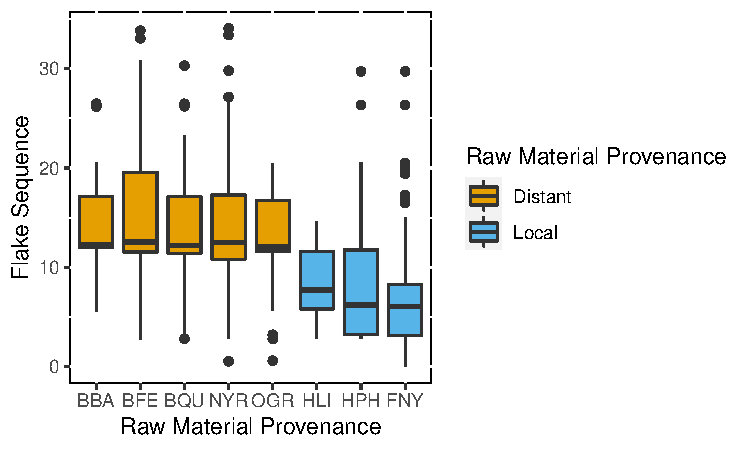
\includegraphics{Reeves_Braun_et_al_2020_Kanjera_South_JHE_files/figure-latex/unnamed-chunk-5-1.pdf}
\caption{The distribution of flake sequence values present within the
Kanjera South flake assemblage. The primary differences in flake
sequence values are between materials originating from more distant
sources than those that originate from local sources of stone.
\label{flake_seq_rm}}
\end{figure}

As previously reported (D. R. Braun, Plummer, Ditchfield, et al. 2009),
the Kanjera core assemblage is comprised of a wide variety of
technological types or core reduction strategies. The frequency of core
reduction strategies present shows a significant relationship with the
raw material type (Fishers exact test, p-value: \textless{} .001). In
general, raw materials that derive from more distant sources, are
represented by core reduction strategies that involve a greater number
of core rotations or more complex rotations (i.e.~centripetal flaking,
figure: \ref{core.tech}). Though unifacial and unidirectional reduction
strategies are present in small frequencies, there is a greater
representation of centripetal, bifacial and multifacial exploitation
strategies in materials from more distant origins (Figure:
\ref{core.tech}). On the other hand, local materials such as the
Fenetized Nyanzian (FNY) and Homa Phonolite (HPH) are represented by
greater number of unifacial or uni-directional core reduction strategies
(Figure: \ref{core.tech}). Homa Limestone, runs contrary to this general
pattern. Although Homa Limestone is found in abundance locally, cores
produced on this raw material type are often multi-facially reduced.
However, as is addressed in the discussion this is likely related to the
properties of the raw material itself (D. R. Braun, Plummer, Ditchfield,
et al. 2009). When core reduction intensity is compared according by
core reduction strategy an interesting pattern emerges. Unifacial and
unipolar, core reduction strategies result in less reduction than
strategies that require bifacial, multifacial or polyhedral strategies
(Kruskal Wallis, P-value: \textless{} .001) (Figure: \ref{core.tech}).
In other words, core reduction strategies that require fewer core
rotations, such as unifacial and unidirectional strategies, are less
reduced than those that involve more complex rotation strategies.

\begin{figure}
\centering
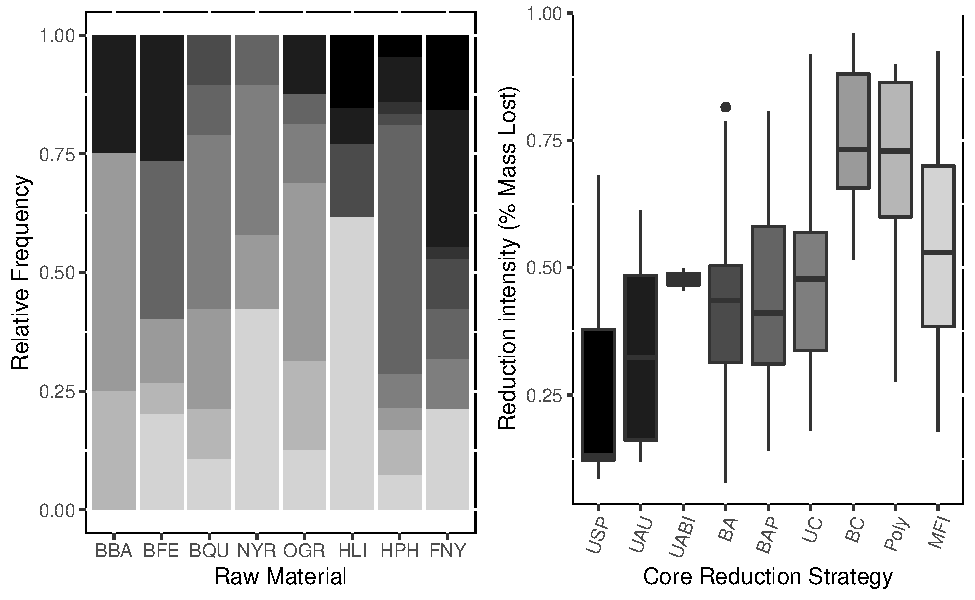
\includegraphics{Reeves_Braun_et_al_2020_Kanjera_South_JHE_files/figure-latex/Figure distribution of core reduction strategies by raw material-1.pdf}
\caption{The distribution of core reduction strategies by raw material
type. With the exception of Homa Limestone, raw materials that derive
from the Kisi highlights more greatly represented by complex core
reduction strategies than those that can be found in the immediate
vicinity of Kanjera South. \textbf{USP}: Unifacial Simple Partial.
\textbf{UAU}: Unidirectional abrupt unifacial. \textbf{UABI}: Unifacial
abrupt bidirectional. \textbf{BA}: Bidirectional Abrupt. \textbf{BAP}
Bifacial Partial. \textbf{UC}: Unifacial centripetal. \textbf{BC}:
Bifacial Centripetal. \textbf{Poly}: Polyhedral. \textbf{MFI}:
Mutifacial Irregular. \label{core.tech}}
\end{figure}

\hypertarget{flake-efficiency}{%
\subsection{Flake efficiency}\label{flake-efficiency}}

Analysis of the relative proportion of edge to mass in flakes indicates
significantly different technological strategies applied to the
different raw materials from the Kanjera South assemblage. Although the
mean values of the different raw materials are relatively similar, the
overall distribution of values indicates that rock types from sources
that are further away from Kanjera South (e.g.~rhyolite, felsite,
quartzite) are produced in a way that allows for much higher efficiency
values than those seen in the rock types found close to Kanjera South.
In particular, the relatively low values seen in the Fenetized Nyanzian
and Homa limestone indicate that flakes made on these rock types were
produced in a manner that does not increase the use life of these cores
(@ D. R. Braun, Rogers, et al. 2008; Shott 1996; Shott and Sillitoe
2004). In particular the differences between the rocks types from the
Kisii highlands (Bukoban quartzite, felsite and basalt) show signficant
differences from those rock types that can be found in the drainages
near Kanjera (e.g.~Homa Limestone and Fenetized Nyanzian,
p\textless{}.01 for all pairwise comparisons between Homa Limestone and
all Bukoban rock types; p\textless{}.001 for all comparisons between
Fenetized Nyanzian and all other rock types Kruskal-Wallis Rank Sum
test, chi2=312.70, df=5, pairwise comparisons between raw materials use
Dunnn's Test with Benjamin-Hochberg correction for multiple
comparisons). It should be noted that even though there are significant
differences between the edge to mass ratios, the distributions show
significant overlap (Figure \textbackslash{}ref\{flake\_efficiency\}.
This indicates that while it is physically possible to produce flakes
with similar edge to mass ratios in each raw material type, hominins at
Kanjera South did not implement this strategy as frequently on raw
materials that were locally abundant. Hominins at Kanjera South
consistently produced flakes with greater edge and less mass from rock
types that came from more distant sources. We only include rock types
that have greater than 50 flakes because the wide variance in values
seen in this measure results in wilidly divergent values in small
samples.

\begin{figure}
\centering
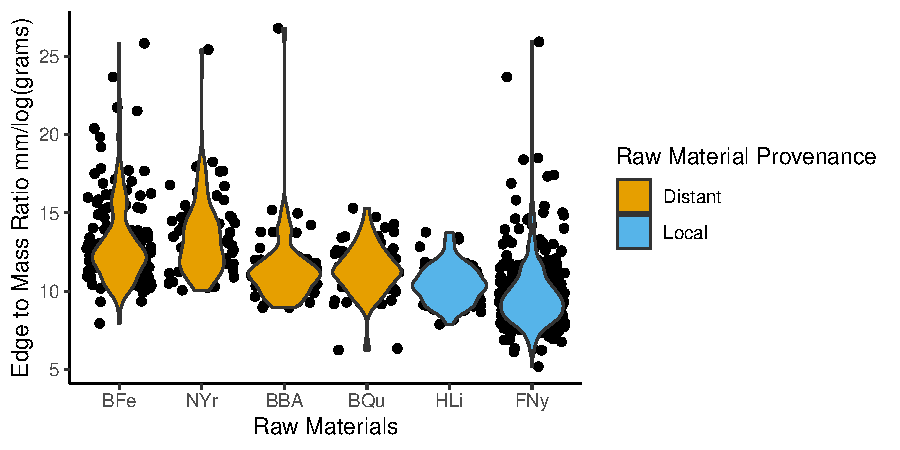
\includegraphics{Reeves_Braun_et_al_2020_Kanjera_South_JHE_files/figure-latex/Figure:Flake Effieciency Data-1.pdf}
\caption{Boxplots of the measures of flake efficiency. Y-axis represents
perimeter of flakes divided by a logarithmically transformed mass value.
\label{flake_efficiency}}
\end{figure}

\hypertarget{discussion}{%
\section{Discussion}\label{discussion}}

\hypertarget{the-influence-of-raw-material-properties}{%
\subsection{The Influence of Raw Material
Properties}\label{the-influence-of-raw-material-properties}}

The results of this study show an interaction between stone tool
utilization, raw material type and core reduction strategies. The most
striking distinction is the difference in the degree of utilization of
materials from local and distant sources. That is, cores that are
derived from the drainages of the more distant Kisi highlands are
significantly more reduced than those from local sources. This is also
reflected in the flake sequence data. Within the Kanjera South flake
assemblage, those produced on exotic raw materials are more likely to be
from later in the reduction sequence than flakes from locally sourced
materials (Figure \ref{flake_seq_rm}). This difference can be explained
by a few different factors. Firstly, raw material properties play a role
in causing these differences. The local fenetized rocks (FNy) are often
discarded before complete reduction because of the intersection of
removals with step fractures or preexisting internal fracture planes
present in the highly metasomatized rocks (D. R. Braun, Plummer,
Ferraro, et al. 2009). The chalky nature and block-like geometry of Homa
limestone (HLi) also limits the number of flakes that can be removed. In
contrast, the majority of raw materials from more distant sources
possess fewer flaws and fracture more predictably than those found
locally (D. R. Braun, Plummer, Ferraro, et al. 2009).

However, differences in material properties do not explain all of the
differences in reduction intensity between local and exotic materials.
If all of the cores that were discarded due to presence of internal
flaws are removed from the assemblage (figure \ref{core.tech}), the
overall pattern remains. In addition, Homa phonolite, a local raw
material, does not have the defects common in other local raw materials
but it is still less reduced than the nonlocal raw materials. In
contrast with the other exotic materials, the properties of the Oyugis
granite (OGR) also constrains the removal of flakes. The particularly
coarse grained nature of this rock type alters its fracture pattern. It
is difficult to maintain angles of less than 90 degrees. It is likely
that hominins could only exploit pre-existing angles on these granite
blocks, thus limiting the degree that they could be reduced (D. R.
Braun, Plummer, Ditchfield, et al. 2009). Despite the limitations
imposed by its material properties, Oyugis granite is still more reduced
than any of the local raw materials (figure \ref{core_redux_rm}).
Previous research shows that the exotic raw materials that were
transported to Kanjera South not only fracture more predictably but also
produce flakes with more durable edges (D. R. Braun, Plummer, Ferraro,
et al. 2009; de la Torre 2004; Ludwig and Harris 1998). The need to
reduce relatively lower quality material may be related to the
durability and the efficiency of the produced edges. In other words,
flakes produced on local rock types have shorter use-lives because their
edges dull more quickly. The consequence of this, is that for any given
use, more flakes of a local raw material are required. In this sense,
the high abundance of these materials and the relatively quick dulling
of their cutting edges may explain the high frequency of local raw
materials in the Kanjera South assemblage.

\hypertarget{implications-for-land-use}{%
\subsection{Implications for Land use}\label{implications-for-land-use}}

The stark differences in the degree of core utilization according to raw
material origin also reflects a dynamic hominin land-use system. Flake
sequence values associated with exotic materials are often from later in
the sequence than those associated with local raw materials. This
pattern could indicate that cores from exotic sources were often
utilized prior to their arrival and discard at Kanjera South. The
presence of highly reduced exotic materials in contrast with lightly
reduced local materials may imply that hominins that visited the Homa
Peninsula may have discarded more utilized exotic materials as they
collected materials that were proximal to Kanjera as part of a mobile
toolkit. This pattern has been observed at the site of FxJj 50 from the
Okote Mbr. of the Koobi Fora Fm. (D. R. Braun, Harris, and Maina 2009).
This may further suggest that stone tool acquisition and discard
behavior may relate to the need to maximize the amount of utility
hominins carried with them. \textbf{In this sense, hominins would have
made decisions to discard raw material when opportunities to increase
the amount useable volume was prssent.} The core reduction pattern at
Kanjera South is also consistent with expectations of raw material
procurement and utilization when conditions are neutral. Under neutral
conditions, raw materials from more distant sources will be, on average,
more reduced, than those from local sources (Brantingham 2003; Pop
2016). The fact that cores from more distant sources are more reduced
than those from local sources is consistent with this pattern. This
``distance-decay'' pattern has been observed in numerous archaeological
studies (eg. Blumenschine et al. (2008); Close (1999); Newman (1994);
Toth (1985)). In addition, neutral expectations state that the variance
in tool reduction intensity will decrease with distance from a given
source. In other words, the variance in the amount of stone tool
reduction intensity should be substantially lower in assemblages of
tools from distant sources. The converse is also predicted by the
distance-decay model. Variance in core reduction will be much greater in
local sources.

This prediction of the distance-decay model is not supported by the
Kanjera South data. In contrast, while exotic materials are reduced more
more substantially than local materials, the interquartile ranges of
flake sequence and core reduction measures of assemblages from distant
sources are as wide (or wider) than those associated with local sources.
This argues against a null hypothesis that the patterns seen in the
lithic assemblage at Kanjera South formed under neutral conditions
(i.e.~no intentional attempt to increase the use life of artifacts from
distant sources). It has been hypothesized that deviations from the
neutral model of this nature may arise due to increasingly linear
movements toward specific locations (Brantingham 2003; @ D. R. Braun,
Rogers, et al. 2008). Moreover, subsequent work modeling the influence
of directed movement towards attractors has shown that while a
distance-decay pattern remains visible, tools from earlier stages of
reduction will be over-represented (i.e.~greater variance in reduction)
(Reeves 2019). Thus, the greater than expected range in variance in the
reduction intensity of distantly sourced cores may suggest that hominins
directed their movement to Kanjera South.

The concept that hominins directed their movement toward Kanjera South,
is supported by other archaeological and paleoecological evidence.
Numerous taphonomic studies of the faunal assemblage from Kanjera South
have verified that hominins efficiently exploited small bovids and may
have processed larger carcasses that were scavenged from carnivores.
(Ferraro et al. 2013; Oliver et al. 2019). Use-wear studies that
demonstrate that hominins carried out a variety of resource processing
activities with the stone artifacts that were produced at Kanjera South,
including butchery and the processing of a variety of plants, including
underground storage organs (USOs) (Lemorini et al. 2014, 2019). These
studies attest to the resource rich environment in which Kanjera South
was situated. These resources ultimately made the Kanjera South locale
and the Homa Pennisula an attractive place for hominins, most likely for
centuries given that the finds were made through three meters of
sequence (upper KS-1 through KS-3). Thus, the patterns evinced by this
study are the result of the repeated visitation by hominins over
generations to Kanjera South, and these patterns likely reflect the
broader foraging ecology of Oldowan Tool makers.

\hypertarget{the-interacting-effect-of-land-use-and-material-properties-on-lithic-technology-at-kanjera-south.}{%
\subsection{The interacting effect of land-use and material properties
on lithic technology at Kanjera
South.}\label{the-interacting-effect-of-land-use-and-material-properties-on-lithic-technology-at-kanjera-south.}}

The results of this study may also suggest that tool utilization, raw
material properties and foraging ecology may interact in complex ways
that structure the patterns of artifact variation we see at Oldowan
sites. Kanjera South artifacts include a wide range of reduction
strategies (D. R. Braun, Plummer, Ditchfield, et al. 2009; Plummer,
Bishop, et al. 2009; Plummer et al. 2001; Plummer and Bishop 2016).
These strategies have a similar appearance to the descriptions of tool
forms that have been described in other Oldowan contexts (de la Torre
and Mora 2005). Interestingly the different reduction strategies present
at Kanjera South seem to be related to reduction intensity. Cores that
are described as having bifacial, multifacial and/or centripetal
patterns of removals exhibit high levels of reduction. Few of the
unifacial cores and partial bifacial cores show this increased level of
reduction intensity (Figure \ref{core.tech}). It could be argued that
this pattern is a consequence of the predictive model used to estimate
core reduction intensity. The reduction intensity model predicts higher
reduction intensity as core rotation increases. This is a pattern that
has been identified in some experimental models of Oldowan core
reduction (Douglass et al. 2017). However, this is not necessarily the
case. Despite the fact that cores produced on Oyugis Granite and Homa
Limestone are often irregular and multi-facial, the predictive model
still discriminates between different levels of reduction in these
cores. Complimentary support can be found in the flakes made from these
raw materials. Flakes made from exotic cores exhibit flake sequence
values that suggest they were produced from later in the flaking
sequence. This independent line of evidence suggests that the predictive
model of core reduction is not over estimated due to rotation. Rather,
this model of reduction intensity is accurately identifying estimates of
the length of core use life in these exotic cores. Therefore it is
possible to examine the representation of various core reduction
strategies in terms of raw material properties and land-use.

The representation of reduction strategies in each raw materials type
also follows the interaction between raw material properties and broader
land-use that is described above. Raw material properties have been
shown to influence reduction intensity decisions previously (D. R.
Braun, Plummer, Ditchfield, et al. 2009). The frequent application of
unifacial reduction strategies to the locally obtained FNy may result
from the limitations imposed by the internal flaws often present in the
rock. In other words, hominins may have only been able to exploit a
single surface on these metasomatized rocks before the knapping process
encountered an internal flaw. Rather than attempt to overcome the flaw
by rotating the core, the high abundance of FNy at KJS may have made it
easier to simply discard the core and acquire a new nodule. High discard
rates in contexts of abundant raw material has been observed in numerous
archaeological and ethnographic contexts (Andrefsky 2008). Moreover, the
technological analysis of the cores suggests that the high
representation of irregular multi-facial cores produced in Homa
Limestone (HLi) and Oyugis Granite (OGr) are the result of continuous
core rotation to exploit naturally occurring angles (D. R. Braun,
Plummer, Ditchfield, et al. 2009). The exploitation of naturally
occurring angles in rocks is a fairly common feature of Oldowan
hominins. (Delagnes and Roche 2005). Yet these mechanical issues do not
explain all of the patterns seen at Kanjera South. Homa phonolite is one
of the most homogeneous raw materials found at Kanjera South. Hominins
at Kanjera South frequently implemented bifacial reduction strategy in
these cores. It was possible to implement longer reduction chains in
this material than was possible with the other local materials. Yet the
these cores are never reduced to the same degree as that seen in the
exotic raw materials.

The cores produced on raw materials from the area surrounding Kanjera
South (i.e.~local materials) exhibit an even representation of various
core reduction strategies. The same pattern is not seen in rocks
transported over large distances. Exotic raw materials show a strong
bias toward more reduced, complete bifacial and multifacial reduction
strategies (Figure \ref{core.tech}). While the HPh shows a high
frequency of bifacial reduction, this reduction is only partial (Figure
\ref{core.tech}). Moreover, cores with multi-facial or centripetal
flaking strategies are seldom produced on Homa Phonolite (Figure
\ref{core.tech}). This contrasts sharply with the prevalence of more
intense core reduction strategies involving greater degrees of core
rotation in rock types from further sources (e.g.~Bukoban Quartzite).
This suggests that raw material properties is not the only factor
influencing core reduction strategies.

The results of the edge-to-mass ratio data suggest that hominins applied
a strategy that more efficiently produced flakes on rock types
transported from greater distances from Kanjera South. In addition,
previous research shows that exotic raw materials also produce more
durable cutting edges (D. R. Braun, Plummer, Ferraro, et al. 2009).
These two factors may have incentivized the retention of exotic raw
materials within the hominin tool-kit. The stock of these ``high
quality'' raw materials would have become increasingly more expensive
(i.e.~in time and energy) to rejuvenate as hominins moved away from the
Kisi highlands (D. R. Braun, Ditchfield, et al. 2008). In this light,
the high frequency of the bifacial and multifacial reduction strategies
may have arisen from a need to maximize the amount utility that could be
extracted from these cores. The exploitation of multiple flake removal
surfaces on a core allows a core to remain active in a toolkit for a
longer period of time. In later times hominins more frequently retouched
formalized tools when the availability of raw materials becomes scarce
(Clark and Barton 2017). In a similar sense, the application of complete
bifacial and multifacial strategies may have allowed hominins to utilize
these high quality exotic materials longer to optimize resource
acquisition at Kanjera South.

It could be argued that this pattern reflects the high level planning
and foresight required to utilize and transport tools within this
dynamic system. However, simpler explanations should also be considered.
Modeling work has shown that tools will inevitably become more utilized
as they are transported from the source, even under neutral or random
conditions (Brantingham 2003; Pop 2016; Reeves 2019). Experimental
research has also shown that the wide range of formal types defined by
Leakey (1971) could arise through a least effort flaking strategy (Toth
1985, 1982). More recently, Moore and Perston (2016) showed cores will
eventually become bifacial or even multi-facial when the flaking
procedure is systematically randomized. Thus, it may be possible to
produce the differences in reduction intensity and reduction strategies
observed between local and exotic materials by simply combining the
influence of simple flaking procedures, stone tool transport, and raw
material selection. Given the relationship between core reduction
patterns and stone tool reduction intensity, the data from Kanjera South
may suggest that different reduction strategies reflect different points
on a reduction continuum rather than intentionally imposed strategies or
socially mediated patterns of production. A similar notion has been
proposed from LCT variability (Iovita and McPherron 2011). Oldowan
researchers must consider the possibility that, in some cases, Oldowan
core variability arises due to an interaction of simple flaking rules
with broader ecological parameters. In this sense, some Oldowan core
variation may be an emergent phenomenon, rather than a direct reflection
of the intentions or information that was transmitted to the knapper.

\hypertarget{implications-for-the-oldowan-as-a-whole.}{%
\section{Implications for the Oldowan as a
whole.}\label{implications-for-the-oldowan-as-a-whole.}}

The site of Kanjera South is unique in relation to Oldowan sites of a
similar age or older. Many of the sites 2 million years old or older are
situated in close proximity to raw materials sources and are comprised
of a singular reduction strategy (Roche, Blumenschine, and Shea 2009;
Plummer and Finestone 2018). In contrast, the assemblage at Kanjera
South shows a substantial representation of exotic raw materials and a
diversity of different core reduction strategies. The results from
Kanjera South elucidate how the interaction of raw material properties,
foraging ecology, and landscape scale constraints on raw material
availability influence technological variability in the Oldowan. While
many sites show strong selection for specific materials, the frequent
use of unifacial reduction strategies at sites such as Lokalelei 2C,
East Gona, Hadar, Omo, Ledi Geraru may relate to the overall abundance
of knappable material that is immediately available at these site (Braun
et al. 2019; Kimbel et al. 1996; Roche et al. 1999; Stout et al. 2005).
In other words, there maybe little incentive to exhaustively reduce a
core when material is so abundant (Clark and Barton 2017).

Kanjera South is also the only site from this time frame that is
situated in an open grassland (Plummer, Ditchfield, et al. 2009). Humans
tend to travel farther and more frequently in open arid environments
than those that live in more productive environments (Burnside et al.
2012). Moreover savanna adapted Chimpanzees from Fongoli also possess a
larger home range and practice fission-fusion less frequently (Pruetz
and Bertolani 2009). If this was also the case for the hominins at
Kanjera South, these factors may have required new technological
strategies in order to accommodate expanded home range sizes. On a
broader scale the technological diversity represented at Kanjera South
may reflect adaptations to the specific contextual conditions at this
locale. The stimulus for increasing the use lives of cores (through
reduction intensity and efficient use of raw material) at Kanjera South
may have been foraging activities that quickly dulled artifact edges
(e.g., butchery and USO processing) (D. R. Braun, Ditchfield, et al.
2008; Lemorini et al. 2014) that were more frequently carried out in
open habitats (Ferraro et al. 2013; Lemorini et al. 2019; Plummer,
Bishop, et al. 2009).

Finally while the preceding analysis emphasizes the role of the broader
environment and land-use on technological variability, ecology is not
the sole driver of Oldowan technical variation. The inter-quartile
ranges in figure \ref{core.tech} show a substantial amount of overlap
between the reduction intensity and core reduction strategies. This
suggests, that not all variation can be explained by environmental
parameters such as raw material avalaibility and material properties.
Moreover, inter-site differences between West Turkana sites are not
easily explained factors such as raw material availability alone (Roche
et al. 2018). This unexplained variation may be the result of
socio-cultural dynamics that may have maintained information regarding
the stone tool production process between groups. However, the fidelity
and the mechanisms that underlie the maintenance of this information
remain an open debate (Hovers 2012; Morgan et al. 2015; Stout et al.
2019; Tennie et al. 2017, 2016). However, the results of this analysis
show that it may be counterproductive for research on Oldowan technology
to focus on specific aspects of stone tool technology (Figure
\ref{variation}). Rather studies should examine the Oldowan within the
broader socio-ecological system. It may be the interaction between
function, ecology and sociality that provide information on the cultural
capacity of Oldowan tool makers.

\hypertarget{conclusion}{%
\section{Conclusion}\label{conclusion}}

Despite the superficial simplicity of the Oldowan, its variability
reflects a complex interconnection of ecological, behavioral and social
factors. These factors are inextricably linked even though researchers
often study them components in isolation. The lithic assemblage from
Kanjera South provides an excellent opportunity to examine the
interacting effects of raw material properties, provenance and
availability of rock types and presumably social variation in the form
of Oldowan artifacts. This is especially important given the context of
other information we have from Kanjera that indicates that hominins
butchered multiple small animals at this site and engaged in other
subsistence strategies. Combination of quantitive measures of stone tool
reduction with qualitative characterizations of lithic technology (e.g
D. R. Braun, Plummer, Ditchfield, et al. (2009); Plummer and Bishop
(2016)) provides new insights into the ecological factors that influence
oldowan technology, and hominin behavior.

The fact that exotic materials are much more substantially reduced that
from local sources reflects the differences in the quality of the raw
materials available. The higher quality of the exotic materials would
have incetivized the transport of these materials over longer distances.
In this light, these differences in reduction also highlight that
Oldowan tools were part of a mobile tool kit that reflects a broader
land-use strategy. The marked differences in reduction intensity in
combination with the paucity of early sequence flakes also suggests that
exotic materials were often utilized prior to their arrival at Kanjera
south. Although exotic materials are more reduced than local marerials
the variance in the amount of stone tool reduction exhibited in the
Kanjera South assemblage does not adhere to neutral expectations. This
result suggests that the lithic assemblage at Kanjera South reflects a
structured land-use pattern, that may indicate that hominins directed
their movement, at least on occassion, to Kanjera South.

This pattern also appears to have an influence on the technological
strategies employed by Oldowan tool makers at Kanjera South. The
relationship between core reduction strategies and reduction intensity
indicates that raw material quality and provenance have a strong
influence on the technological variation observed within a lithic
assemblage. While these results show that ecological parameters have a
strong effect on stone tool variation, a substantial amount of variation
remains unexplained by ecology alone. Overall, these results suggest
that future studies must utilize a more integrated approach to
understand the behavioral significance of the Oldowan.

\hypertarget{references}{%
\section*{References}\label{references}}
\addcontentsline{toc}{section}{References}

\hypertarget{refs}{}
\leavevmode\hypertarget{ref-andrefskyRawMaterialAvailabilityOrganization2008}{}%
Andrefsky, William. 2008. ``Raw-Material Availability and the
Organization of Technology.'' \emph{Amerian Antiquity} 59 (1): 21--34.

\leavevmode\hypertarget{ref-andrefskyAnalysisStoneTool2009}{}%
---------. 2009. ``The Analysis of Stone Tool Procurement, Production,
and Maintenance.'' \emph{Journal of Archaeological Research} 17 (1):
65--103. \url{https://doi.org/10.1007/s10814-008-9026-2}.

\leavevmode\hypertarget{ref-bamforthSettlementRawMaterial1990}{}%
Bamforth, Douglas B. 1990. ``Settlement, Raw Material, and Lithic
Procurement in the Central Mojave Desert.'' \emph{Journal of
Anthropological Archaeology} 9 (1): 70--104.
\url{https://doi.org/10.1016/0278-4165(90)90006-Y}.

\leavevmode\hypertarget{ref-bamforthTechnologicalEfficiencyTool1986}{}%
Bamforth, Douglas B. 1986. ``Technological Efficiency and Tool
Curation.'' \emph{American Antiquity} 51 (1): 38--50.
\url{https://doi.org/10.2307/280392}.

\leavevmode\hypertarget{ref-barhamFirstAfricansAfrican2008}{}%
Barham, Lawrence, and Peter Mitchell. 2008. \emph{The First Africans:
African Archaeology from the Earliest Tool Makes to Most Recent
Foragers}. Cambridge University Press.

\leavevmode\hypertarget{ref-behrensmeyerPleistoceneLocalityKanjera1995}{}%
Behrensmeyer, A. K., R. Potts, Thomas W. Plummer, L. Tauxe, N. Opdyke,
and T. Jorstad. 1995. ``The Pleistocene Locality of Kanjera, Western
Kenya: Stratigraphy, Chronology and Paleoenvironments.'' \emph{Journal
of Human Evolution} 29 (3): 247--74.
\url{https://doi.org/10.1006/jhev.1995.1059}.

\leavevmode\hypertarget{ref-binfordContemporaryModelBuilding1976}{}%
Binford, Lewis R. 1976. ``Contemporary Model Building: Paradigms and the
Current State of Palaeolithic Research.'' In \emph{Models in
Archaeology}, edited by David L. Clarke, 18. London: Routledge.
\url{https://doi.org/10.1590/S1516-18462008000300012}.

\leavevmode\hypertarget{ref-binfordConstructingFramesReference2001}{}%
---------. 2001. \emph{Constructing Frames of Reference}. San Fransisco:
University of California Press.

\leavevmode\hypertarget{ref-bishopRecentResearchOldowan2006}{}%
Bishop, Laura C., Thomas W. Plummer, Joseph V. Ferraro, David R. Braun,
Peter W. Ditchfield, Fritz Hertel, John D. Kingston, Jason Hicks, and
Richard Potts. 2006. ``Recent Research into Oldowan Hominin Activities
at Kanjera South , Western Kenya.'' \emph{African Archaeological Review}
23: 31--40. \url{https://doi.org/10.1007/s10437-006-9006-1}.

\leavevmode\hypertarget{ref-blumenschineArchaeologicalPredictionsHominid1998}{}%
Blumenschine, R.J., and C.R. Peters. 1998. ``Archaeological Predictions
for Hominid Land Use in the Paleo-Olduvai Basin, Tanzania, During
Lowermost Bed II Times.'' \emph{Journal of Human Evolution} 34 (6):
565--607. \url{https://doi.org/10.1006/jhev.1998.0216}.

\leavevmode\hypertarget{ref-blumenschineEffectsDistanceStone2008}{}%
Blumenschine, Robert J., Fidelis T. Masao, Joanne C. Tactikos, and James
I. Ebert. 2008. ``Effects of Distance from Stone Source on
Landscape-Scale Variation in Oldowan Artifact Assemblages in the
Paleo-Olduvai Basin, Tanzania.'' \emph{Journal of Archaeological
Science} 35 (1): 76--86.
\url{https://doi.org/10.1016/j.jas.2007.02.009}.

\leavevmode\hypertarget{ref-blumenschineOlduvaiGorgeOlduvai2012}{}%
Blumenschine, Robert J., Ian G. Stanistreet, and Fidelis T. Masao. 2012.
``Olduvai Gorge and the Olduvai Landscape Paleoanthropology Project.''
\emph{Journal of Human Evolution} 63 (2): 247--50.
\url{https://doi.org/10.1016/j.jhevol.2012.05.005}.

\leavevmode\hypertarget{ref-brantinghamMobilityCompetitionPlioPleistocene1998}{}%
Brantingham, P. Jeffrey. 1998. ``Mobility, Competition, and
Plio-Pleistocene Hominid Foraging Groups.'' \emph{Journal of
Archaeological Method and Theory} 5 (1): 57--98.
\url{https://doi.org/10.1007/BF02428416}.

\leavevmode\hypertarget{ref-brantinghamNeutralModelStone2003}{}%
---------. 2003. ``A Neutral Model of Stone Raw Material Procurement.''
\emph{American Antiquity} 68 (3): 487--509.
\url{https://doi.org/10.2307/3557105}.

\leavevmode\hypertarget{ref-brantinghamConstraintsLevalloisCore2001}{}%
Brantingham, P. Jeffrey, and Steven L Kuhn. 2001. ``Constraints on
Levallois Core Technology: A Mathematical Model.'' \emph{Journal of
Archaeological Science} 28 (7): 747--61.
\url{https://doi.org/10.1006/jasc.2000.0594}.

\leavevmode\hypertarget{ref-braunEarliestKnownOldowan2019}{}%
Braun, David R., Vera Aldeias, Will Archer, J. Ramon Arrowsmith, Niguss
Baraki, Christopher J. Campisano, Alan L. Deino, et al. 2019. ``Earliest
Known Oldowan Artifacts at \&Gt;2.58 Ma from Ledi-Geraru, Ethiopia,
Highlight Early Technological Diversity.'' \emph{Proceedings of the
National Academy of Sciences} 116 (24): 11712--7.
\url{https://doi.org/10.1073/pnas.1820177116}.

\leavevmode\hypertarget{ref-braunOldowanBehaviorRaw2008}{}%
Braun, David R., Peter Ditchfield, Joseph V. Ferraro, David Maina, Laura
C. Bishop, and Richard Potts. 2008. ``Oldowan Behavior and Raw Material
Transport: Perspectives from the Kanjera Formation.'' \emph{Journal of
Archaeological Science} 35 (8): 2329--45.
\url{https://doi.org/10.1016/j.jas.2008.03.004}.

\leavevmode\hypertarget{ref-braunTechnologicalDevelopmentsOldowan2003}{}%
Braun, David R., and Jack W.K. Harris. 2003. ``Technological
Developments in the Oldowan of Koobi Fora: Innovative Techniques of
Artifact Analysis.'' In, 29.

\leavevmode\hypertarget{ref-braunOldowanRawMaterial2009}{}%
Braun, David R., John W.K. Harris, and David N. Maina. 2009. ``Oldowan
Raw Material Procurement and Use: Evidence from the Koobi Fora
Formation.'' \emph{Archaeometry} 51: 26--42.

\leavevmode\hypertarget{ref-braunOldowanTechnologyRaw2009}{}%
Braun, David R., Thomas W. Plummer, Peter W. Ditchfield, Laura C.
Bishop, and Joseph V. Ferraro. 2009. ``Oldowan Technology and Raw
Material Variability at Kanjera South.'' In \emph{Interdisciplinary
Approaches to the Oldowan}, 99--110. Vertebrate Paleobiology and
Paleoanthropology. Dordrecht: Springer Netherlands.
\url{https://doi.org/10.1007/978-1-4020-9060-8_9}.

\leavevmode\hypertarget{ref-braunRawMaterialQuality2009}{}%
Braun, David R., Thomas W. Plummer, Joseph V. Ferraro, Peter Ditchfield,
and Laura C. Bishop. 2009. ``Raw Material Quality and Oldowan Hominin
Toolstone Preferences: Evidence from Kanjera South, Kenya.''
\emph{Journal of Archaeological Science} 36 (7): 1605--14.
\url{https://doi.org/10.1016/j.jas.2009.03.025}.

\leavevmode\hypertarget{ref-braunLandscapescaleVariationHominin2008}{}%
Braun, David R., Michael J. Rogers, John W.K. Harris, and Steven J.
Walker. 2008. ``Landscape-Scale Variation in Hominin Tool Use: Evidence
from the Developed Oldowan.'' \emph{Journal of Human Evolution} 55 (6):
1053--63. \url{https://doi.org/10.1016/j.jhevol.2008.05.020}.

\leavevmode\hypertarget{ref-braunOldowanReductionSequences2008}{}%
Braun, David R., Joanne C. Tactikos, Joseph V. Ferraro, Shira L. Arnow,
and John W.K. Harris. 2008. ``Oldowan Reduction Sequences:
Methodological Considerations.'' \emph{Journal of Archaeological
Science} 35 (8): 2153--63.
\url{https://doi.org/10.1016/j.jas.2008.01.015}.

\leavevmode\hypertarget{ref-bunnFxJj50EarlyPleistocene1980}{}%
Bunn, Henry, John W.K. Harris, Glynn Isaac, Zefe Kaufulu, Ellen Kroll,
Kathy Schick, Nicholas Toth, and Anna K. Behrensmeyer. 1980. ``FxJj50:
An Early Pleistocene Site in Northern Kenya.'' \emph{World Archaeology}
12 (2): 109--36. \url{https://doi.org/10.1080/00438243.1980.9979787}.

\leavevmode\hypertarget{ref-burnsideHumanMacroecologyLinking2012}{}%
Burnside, William R., James H. Brown, Oskar Burger, Marcus J. Hamilton,
Melanie Moses, and Luis M.A. Bettencourt. 2012. ``Human Macroecology:
Linking Pattern and Process in Big-Picture Human Ecology.''
\emph{Biological Reviews} 87 (1): 194--208.
\url{https://doi.org/10.1111/j.1469-185X.2011.00192.x}.

\leavevmode\hypertarget{ref-chavaillonDecouverteNiveauOldowayen1970}{}%
Chavaillon, Jean. 1970. ``Découverte d'un niveau oldowayen dans la basse
vallée de l'Omo (Ethiopie).'' \emph{Bulletin de La Société Préhistorique
Française} 67 (1). Société Préhistorique Française: 7--11.
\url{https://doi.org/10.3406/bspf.1970.10428}.

\leavevmode\hypertarget{ref-clarkLithicsLandscapesLongueduree2017}{}%
Clark, G. A., and C. Michael Barton. 2017. ``Lithics, Landscapes \& La
Longue-Durée \& Expediency as Expressions of Forager Mobility.''
\emph{Quaternary International} 450: 137--49.
\url{https://doi.org/10.1016/j.quaint.2016.08.002}.

\leavevmode\hypertarget{ref-clarkAfricaPrehistoryPeripheral1975}{}%
Clark, J. Desmond. 1975. ``Africa in Prehistory: Peripheral or
Paramount?'' \emph{Man} 10 (2). {[}Wiley, Royal Anthropological
Institute of Great Britain and Ireland{]}: 175--98.
\url{https://doi.org/10.2307/2800493}.

\leavevmode\hypertarget{ref-clarksonMeasuringCoreReduction2013}{}%
Clarkson, Chris. 2013. ``Measuring Core Reduction Using 3D Flake Scar
Density: A Test Case of Changing Core Reduction at Klasies River Mouth,
South Africa.'' \emph{Journal of Archaeological Science} 40 (12):
4348--57. \url{https://doi.org/10.1016/j.jas.2013.06.007}.

\leavevmode\hypertarget{ref-closeDistanceDecayUneasy1999}{}%
Close, Angela E. 1999. ``Distance and Decay: An Uneasy Relationship.''
\emph{Antiquity} 73 (279): 24--32.
\url{https://doi.org/10.1017/S0003598X00087810}.

\leavevmode\hypertarget{ref-cotterellEssentialMechanicsConchoidal1985}{}%
Cotterell, B., J. Kamminga, and F. P. Dickson. 1985. ``The Essential
Mechanics of Conchoidal Flaking.'' \emph{International Journal of
Fracture} 29 (4): 205--21. \url{https://doi.org/10.1007/BF00125471}.

\leavevmode\hypertarget{ref-daviesModelingRelationshipsSpace2018}{}%
Davies, Benjamin, Simon J Holdaway, and Patricia C Fanning. 2018.
``Modeling Relationships Between Space, Movement, and Lithic Geometric
Attributes.'' \emph{Amerian Antiquity} American A: 1--18.
\url{https://doi.org/10.1017/aaq.2018.23}.

\leavevmode\hypertarget{ref-delagnesLatePlioceneHominid2005}{}%
Delagnes, A, and H Roche. 2005. ``Late Pliocene Hominid Knapping Skills:
The Case of Lokalalei 2C, West Turkana, Kenya.'' \emph{Journal of Human
Evolution} 48 (5): 435--72.
\url{https://doi.org/10.1016/j.jhevol.2004.12.005}.

\leavevmode\hypertarget{ref-delatorreOmoRevisitedEvaluating2004}{}%
de la Torre, Ignacio. 2004. ``Omo Revisited: Evaluating the
Technological Skills of Pliocene Hominids.'' \emph{Current Anthropology}
45 (4): 439--65. \url{https://doi.org/10.1086/422079}.

\leavevmode\hypertarget{ref-delatorreTechnologicalStrategiesLower2005}{}%
de la Torre, Ignacio, and Rafael Mora. 2005. \emph{Technological
Strategies in the Lower Pleistocene at Olduvai Beds I and II}. Liege:
Service de Prehistoire, Universite de Liege.

\leavevmode\hypertarget{ref-delatorreignacioEarlyStoneAge2011}{}%
de la Torre Ignacio, I. 2011. ``The Early Stone Age Lithic Assemblages
of Gadeb (Ethiopia) and the Developed Oldowan/Early Acheulean in East
Africa.'' \emph{Journal of Human Evolution} 60 (6): 768--812.
\url{https://doi.org/10.1016/j.jhevol.2011.01.009}.

\leavevmode\hypertarget{ref-dibbleMiddlePaleolithicScraper1995}{}%
Dibble, Harold. 1995. ``Middle Paleolithic Scraper Reduction:
Background, Clarification, and Review of the Evidence to Date.''
\emph{Journal of Archaeological Method and Theory} 2 (4): 299--368.

\leavevmode\hypertarget{ref-ditchfieldGeochronologyPhysicalContext2018}{}%
Ditchfield, P. W., E. Whitfield, T. Vincent, Thomas W. Plummer, David R.
Braun, Alan L. Deino, J. S. Oliver, J. Louys, and Laura C. Bishop. 2018.
``Geochronology and Physical Context of Oldowan Site Formation at
Kanjera South, Kenya.'' \emph{Geological Magazine}, 1--11.
\url{https://doi.org/10.1017/S0016756818000602}.

\leavevmode\hypertarget{ref-dogandzicEdgeLengthSurface2015}{}%
Dogandži\a'c, Tamara, David R. Braun, and Shannon P. McPherron. 2015.
``Edge Length and Surface Area of a Blank: Experimental Assessment of
Measures, Size Predictions and Utility.'' \emph{PLoS ONE} 10 (9).
\url{https://doi.org/10.1371/journal.pone.0133984}.

\leavevmode\hypertarget{ref-douglassArchaeologicalPotentialInformal2010}{}%
Douglass, Matthew J. 2010. ``The Archaeological Potential of Informal
Lithic Technologies: A Case Study of Assemblage Variability in Western
New South Wales, Australia.'' PhD Thesis, Auckland: University of
Auckland.

\leavevmode\hypertarget{ref-douglassCoreUseLifeDistributions2017}{}%
Douglass, Matthew J., Sam C. Lin, David R. Braun, and Thomas W. Plummer.
2017. ``Core Use-Life Distributions in Lithic Assemblages as a Means for
Reconstructing Behavioral Patterns.'' \emph{Journal of Archaeological
Method and Theory}, 1--35.
\url{https://doi.org/10.1007/s10816-017-9334-2}.

\leavevmode\hypertarget{ref-erenAreUpperPaleolithic2008}{}%
Eren, Metin I., Aaron Greenspan, and C. Garth Sampson. 2008. ``Are Upper
Paleolithic Blade Cores More Productive Than Middle Paleolithic
Discoidal Cores? A Replication Experiment.'' \emph{Journal of Human
Evolution} 55 (6): 952--61.
\url{https://doi.org/10.1016/j.jhevol.2008.07.009}.

\leavevmode\hypertarget{ref-erenKuhnGeometricIndex2009}{}%
Eren, Metin I., and C. Garth Sampson. 2009. ``Kuhn's Geometric Index of
Unifacial Stone Tool Reduction (GIUR): Does It Measure Missing Flake
Mass?'' \emph{Journal of Archaeological Science} 36 (6): 1243--7.
\url{https://doi.org/10.1016/j.jas.2009.01.011}.

\leavevmode\hypertarget{ref-ferraroEarliestArchaeologicalEvidence2013}{}%
Ferraro, Joseph V., Thomas W. Plummer, Briana L. Pobiner, James S.
Oliver, Laura C. Bishop, David R. Braun, Peter W. Ditchfield, et al.
2013. ``Earliest Archaeological Evidence of Persistent Hominin
Carnivory.'' \emph{PLOS ONE} 8 (4): e62174.
\url{https://doi.org/10.1371/journal.pone.0062174}.

\leavevmode\hypertarget{ref-foleyModelRegionalArchaeological1981}{}%
Foley, Robert. 1981a. ``A Model of Regional Archaeological Structure.''
\emph{Proceedings of the Prehistoric Society} 1-17: 1--17.

\leavevmode\hypertarget{ref-foleyOffsiteArchaeologyAlternative1981}{}%
---------. 1981b. ``Off-Site Archaeology: An Alternative Approach for
the Short-Sited.'' In \emph{Pattern of the Past: Studies in Honour of
David Clarke}, 33:139--53. Cambridge: Cambridge University Press.

\leavevmode\hypertarget{ref-gallottiAcheuleanEastAfrica2018}{}%
Gallotti, Rosalia. 2018. ``Before the Acheulean in East Africa: An
Overview of the Oldowan Lithic Assemblages.'' In \emph{The Emergence of
the Acheulean in East Africa and Beyond}, edited by Rosalia Gallotti and
Margherita Mussi, 13--32. Cham: Springer International Publishing.
\url{https://doi.org/10.1007/978-3-319-75985-2_2}.

\leavevmode\hypertarget{ref-harmandVariabilityRawMaterial2009}{}%
Harmand, Sonia. 2009. ``Variability in Raw Material Selectivity at the
Late Pliocene Sites of Lokalalei, West Turkana, Kenya.'' In
\emph{Interdisciplinary Approaches to the Oldowan}, edited by Erella
Hovers and David R. Braun, 85--97. Dordrecht: Springer Netherlands.
\url{https://doi.org/10.1007/978-1-4020-9060-8_8}.

\leavevmode\hypertarget{ref-harrisKarariIndustryIts1978}{}%
Harris, John William Kendal. 1978. ``The Karari Industry, Its Place in
East African Prehistory.'' PhD Thesis, Univversity of California,
Berkeley.

\leavevmode\hypertarget{ref-hayGeologyOlduvaiGorge1976}{}%
Hay, Richard LeRoy. 1976. \emph{Geology of the Olduvai Gorge}. Los
Angeles: University of California Press.

\leavevmode\hypertarget{ref-holdawayRecordStoneStudy2004}{}%
Holdaway, Simon, Nicola Stern, and Parth R. Chauhan. 2004. ``A Record in
Stone. The Study of Australia's Flaked Stone Artefacts.''

\leavevmode\hypertarget{ref-hoversInventionReinventionInnovation2012}{}%
Hovers, Erella. 2012. ``Invention, Reinvention and Innovation.'' In
\emph{Developments in Quaternary Sciences}, 16:51--68. Elsevier.
\url{https://doi.org/10.1016/B978-0-444-53821-5.00005-1}.

\leavevmode\hypertarget{ref-inizanTechnologyTerminologyKnapped1999}{}%
Inizan, Marie-Louise, Mich\a`ele Reduron-Ballinger, H\a'el\a`ene Roche,
Jacques Tixier, and Jehanne F\a'eblot-Augustins, eds. 1999.
\emph{Technology and Terminology of Knapped Stone: Followed by a
Multilingual Vocabulary - Arabic, English, French, German,Greek,
Italian, Portuguese, Spanish}. Préhistoire de La Pierre Taillée 5.
Nanterre: CREP.

\leavevmode\hypertarget{ref-iovitaHandaxeReloadedMorphometric2011}{}%
Iovita, Radu, and Shannon P. McPherron. 2011. ``The Handaxe Reloaded: A
Morphometric Reassessment of Acheulian and Middle Paleolithic
Handaxes.'' \emph{Journal of Human Evolution} 61 (1): 61--74.
\url{https://doi.org/10.1016/j.jhevol.2011.02.007}.

\leavevmode\hypertarget{ref-isaacArchaeologyHumanOrigins1984}{}%
Isaac, Glynn. 1984. ``The Archaeology of Human Origins: Studies of the
Lower Pleistocene in East Africa, 1971-1981.'' In \emph{Advances in
World Archaeology}, 1--86.

\leavevmode\hypertarget{ref-isaacStoneAgeVisiting1981}{}%
Isaac, Glynn Ll. 1981. ``Stone Age Visiting Cards: Approaches to the
Study of Early Land Use Patterns.'' In \emph{Pattern of the Past:
Studies in Honour of David Clarke}, 131--55. Cambridge: University of
Cambridge Press.

\leavevmode\hypertarget{ref-isaacBonesContentionCompeting1983}{}%
Isaac, Glynn L.L. 1983. ``Bones in Contention: Competing Explanations
for the Juxtaposition of Early Pleistocene Artefacts and Faunal
Remains.'' In \emph{Animals in ArchaeoloftL Hunters and Their Prey},
3--19. Oxford: British Archaeological Reports.

\leavevmode\hypertarget{ref-isaacScatterPatches1976}{}%
Isaac, Glynn Ll., and John W.K. Harris. 1976. ``The Scatter Between the
Patches.'' In \emph{The Krober Anthropological Society}. Berkeley:
Unpublished.

\leavevmode\hypertarget{ref-isaacKoobiForaResearch1997}{}%
Isaac, Glynn Llwelyn, and Barbara Isaac. 1997. \emph{Koobi Fora Research
Project. "Koobi Fora Research Project Vol. 5: Plio-Pleistocene
Archaeology}. Oxford: Oxford University Press.

\leavevmode\hypertarget{ref-keeleyMicrowearPolishesEarly1981}{}%
Keeley, Lawrence H., and Nicholas Toth. 1981. ``Microwear Polishes on
Early Stone Tools from Koobi Fora, Kenya.'' \emph{Nature} 293 (5832):
464--65. \url{https://doi.org/10.1038/293464a0}.

\leavevmode\hypertarget{ref-kentPleistoceneBedsKanam1942a}{}%
Kent, P. E. 1942. ``The Pleistocene Beds of Kanam and Kanjera,
Kavirondo, Kenya.'' \emph{Geological Magazine} 79 (2): 117--32.
\url{https://doi.org/10.1017/S001675680007360X}.

\leavevmode\hypertarget{ref-kimbelLatePlioceneHomo1996}{}%
Kimbel, W.H., R.C. Walter, D.C. Johanson, K.E. Reed, J.L. Aronson, Z.
Assefa, C.W. Marean, et al. 1996. ``Late Pliocene Homo and Oldowan Tools
from the Hadar Formation (Kada Hadar Member), Ethiopia.'' \emph{Journal
of Human Evolution} 31 (6): 549--61.
\url{https://doi.org/10.1006/jhev.1996.0079}.

\leavevmode\hypertarget{ref-kuhnWhatMovesUs2016}{}%
Kuhn, Steven L., David A. Raichlen, and Amy E. Clark. 2016. ``What Moves
Us? How Mobility and Movement Are at the Center of Human Evolution.''
\emph{Evolutionary Anthropology} 25 (3): 86--97.
\url{https://doi.org/10.1002/evan.21480}.

\leavevmode\hypertarget{ref-detorreRemarksCurrentTheoretical2009}{}%
la de Torre, Ignacio, and Rafael Mora. 2009. ``Remarks on the Current
Theoretical and Methodological Approaches to the Study of Early
Technological Strategies in Eastern Africa.'' In \emph{Interdisciplinary
Approaches to the Oldowan}, edited by Erella Hovers and David R. Braun,
15--24. Vertebrate Paleobiology and Paleoanthropology. Dordrecht:
Springer Netherlands. \url{https://doi.org/10.1007/978-1-4020-9060-8_2}.

\leavevmode\hypertarget{ref-leakeyOlduvaiGorgeVol1971}{}%
Leakey, Mary. 1971. \emph{Olduvai Gorge Vol. 3 Beds I and II}.
Cambridge: Cambridge University Press.

\leavevmode\hypertarget{ref-lemoriniOldStonesSong2019}{}%
Lemorini, Cristina, Laura C. Bishop, Thomas W. Plummer, David R. Braun,
Peter W. Ditchfield, and James S. Oliver. 2019. ``Old Stones' SongSecond
Verse: Use-Wear Analysis of Rhyolite and Fenetized Andesite Artifacts
from the Oldowan Lithic Industry of Kanjera South, Kenya.''
\emph{Archaeological and Anthropological Sciences} 11 (9): 4729--54.
\url{https://doi.org/10.1007/s12520-019-00800-z}.

\leavevmode\hypertarget{ref-lemoriniOldStonesSong2014}{}%
Lemorini, Cristina, Thomas W. Plummer, David R. Braun, Alyssa N.
Crittenden, Peter W. Ditchfield, Laura C. Bishop, Fritz Hertel, et al.
2014. ``Old Stones' Song: Use-Wear Experiments and Analysis of the
Oldowan Quartz and Quartzite Assemblage from Kanjera South (Kenya).''
\emph{Journal of Human Evolution} 72 (July): 10--25.
\url{https://doi.org/10.1016/j.jhevol.2014.03.002}.

\leavevmode\hypertarget{ref-linUtilityEconomizationUnretouched2013}{}%
Lin, Sam C., Zeljko Rezek, David Braun, and Harold L. Dibble. 2013. ``On
the Utility and Economization of Unretouched Flakes: The Effects of
Exterior Platform Angle and Platform Depth.'' \emph{American Antiquity}
78 (4): 724--45. \url{https://doi.org/10.2307/43184970}.

\leavevmode\hypertarget{ref-ludwigTechnologicalReassessmentEast1998}{}%
Ludwig, Brian V, and J W K Harris. 1998. ``Towards a Technological
Reassessment of East African Plio-Pleistocene Lithic Assemblages.'' In
\emph{Early Human Behavior in Global Context: The Rise of Diversity of
the Lower Palaeolithic Period}, edited by Ravi Korisettar and Michael D.
Petraglia, 23. New York: Routledge.

\leavevmode\hypertarget{ref-mooreExperimentalInsightsCognitive2016}{}%
Moore, Mark W., and Yinika Perston. 2016. ``Experimental Insights into
the Cognitive Significance of Early Stone Tools.'' Edited by Michael D.
Petraglia. \emph{PLOS ONE} 11 (7): e0158803.
\url{https://doi.org/10.1371/journal.pone.0158803}.

\leavevmode\hypertarget{ref-morganExperimentalEvidenceCoevolution2015}{}%
Morgan, T. J. H., N. T. Uomini, L. E. Rendell, L. Chouinard-Thuly, S. E.
Street, H. M. Lewis, C. P. Cross, et al. 2015. ``Experimental Evidence
for the Co-Evolution of Hominin Tool-Making Teaching and Language.''
\emph{Nature Communications} 6 (1): 1--8.
\url{https://doi.org/10.1038/ncomms7029}.

\leavevmode\hypertarget{ref-mullerIdentifyingMajorTransitions2016}{}%
Muller, Antoine, and Chris Clarkson. 2016. ``Identifying Major
Transitions in the Evolution of Lithic Cutting Edge Production Rates.''
Edited by Roberto Macchiarelli. \emph{PLOS ONE} 11 (12): e0167244.
\url{https://doi.org/10.1371/journal.pone.0167244}.

\leavevmode\hypertarget{ref-nelsonStudyTechnologicalOrganization1991}{}%
Nelson, Margaret C. 1991. ``The Study of Technological Organization.''
\emph{Archaeological Method and Theory} 3: 57--100.

\leavevmode\hypertarget{ref-newmanEffectsDistanceLithic1994}{}%
Newman, Jay R. 1994. ``The Effects of Distance on Lithic Material
Reduction Technology.'' \emph{Journal of Field Archaeology} 21 (4):
491--501. \url{https://doi.org/10.1179/009346994797175541}.

\leavevmode\hypertarget{ref-oliverBovidMortalityPatterns2019}{}%
Oliver, James S., Thomas W. Plummer, Fritz Hertel, and Laura C. Bishop.
2019. ``Bovid Mortality Patterns from Kanjera South, Homa Peninsula,
Kenya and FLK-Zinj, Olduvai Gorge, Tanzania: Evidence for Habitat
Mediated Variability in Oldowan Hominin Hunting and Scavenging
Behavior.'' \emph{Journal of Human Evolution} 131 (June): 61--75.
\url{https://doi.org/10.1016/j.jhevol.2019.03.009}.

\leavevmode\hypertarget{ref-petersLandscapePerspectivesPossible1995}{}%
Peters, C R, and R J Blumenschine. 1995. ``Landscape Perspectives on
Possible Land Use Patterns for Early Pleistocene Hominids in the Olduvai
Basin, Tanzania.'' \emph{Journal of Human Evolution} 29: 321--62.

\leavevmode\hypertarget{ref-plummerFlakedStonesOld2004}{}%
Plummer, Thomas W. 2004. ``Flaked Stones and Old Bones: Biological and
Cultural Evolution at the Dawn of Technology.'' \emph{Yearbook of
Physical Anthropology} 47: 118--64.
\url{https://doi.org/10.1002/ajpa.20157}.

\leavevmode\hypertarget{ref-plummerOldowanHomininBehavior2016}{}%
Plummer, Thomas W., and Laura C. Bishop. 2016. ``Oldowan Hominin
Behavior and Ecology at Kanjera South, Kenya.'' \emph{Journal of
Anthropological Sciences}, no. 94: 29--40.
\url{https://doi.org/10.4436/JASS.94033}.

\leavevmode\hypertarget{ref-plummerEnvironmentalContextOldowan2009}{}%
Plummer, Thomas W., Laura C. Bishop, Peter W. Ditchfield, Joseph V.
Ferraro, John D. Kingston, Fritz Hertel, and David R. Braun. 2009. ``The
Environmental Context of Oldowan Hominin Activities at Kanjera South,
Kenya.'' In \emph{Interdisciplinary Approaches to the Oldowan}, edited
by Erella Hovers and David R. Braun, 149--60. Vertebrate Paleobiology
and Paleoanthropology. Dordrecht: Springer Netherlands.
\url{https://doi.org/10.1007/978-1-4020-9060-8_12}.

\leavevmode\hypertarget{ref-plummerResearchLatePliocene1999}{}%
Plummer, Thomas W., Laura C. Bishop, Peter W. Ditchfield, and Jason
Hicks. 1999. ``Research on Late Pliocene Oldowan Sites at Kanjera South,
Kenya.'' \emph{Journal of Human Evolution} 36 (2): 151--70.
\url{https://doi.org/10.1006/jhev.1998.0256}.

\leavevmode\hypertarget{ref-plummerOldestEvidenceToolmaking2009}{}%
Plummer, Thomas W., Peter W. Ditchfield, Laura C. Bishop, John D.
Kingston, Joseph V. Ferraro, David R. Braun, Fritz Hertel, and Richard
Potts. 2009. ``Oldest Evidence of Toolmaking Hominins in a
Grassland-Dominated Ecosystem.'' \emph{PLoS ONE} 4 (9).
\url{https://doi.org/10.1371/journal.pone.0007199}.

\leavevmode\hypertarget{ref-plummerLatePlioceneOldowan2001}{}%
Plummer, Thomas W., Joseph Ferraro, Peter Ditchfield, Laura Bishop, and
Richard Potts. 2001. ``Late Pliocene Oldowan Excavations at Kanjera
South, Kenya.'' \emph{Antiquity} 75 (290): 809--10.
\url{https://doi.org/10.1017/S0003598X00089365}.

\leavevmode\hypertarget{ref-plummerArchaeologicalSitesMa2018}{}%
Plummer, Thomas W., and Emma M. Finestone. 2018. ``3 Archaeological
Sites from 2.6 - 2.0 Ma: Toward a Deeper Understanding of the Early
Oldowan.'' In. February.

\leavevmode\hypertarget{ref-popSimulatingLithicRaw2016}{}%
Pop, Cornel M. 2016. ``Simulating Lithic Raw Material Variability in
Archaeological Contexts: A Re-Evaluation and Revision of Brantingham's
Neutral Model.'' \emph{Journal of Archaeological Method and Theory} 23
(4): 1127--61. \url{https://doi.org/10.1007/s10816-015-9262-y}.

\leavevmode\hypertarget{ref-pottsWhyOldowanPlioPleistocene1991}{}%
Potts, Richard. 1991. ``Why the Oldowan? Plio-Pleistocene Toolmaking and
the Transport of Resources.'' \emph{Journal of Anthropological Research}
47 (2): 153--76. \url{https://doi.org/10.1086/jar.47.2.3630323}.

\leavevmode\hypertarget{ref-pruetzChimpanzeePanTroglodytes2009}{}%
Pruetz, Jill, and Paco Bertolani. 2009. ``Chimpanzee (Pan Troglodytes
Verus) Behavioral Responses to Stresses Associated with Living in a
Savannah-Mosaic Environment: Implications for Hominin Adaptations to
Open Habitats.'' \emph{PaleoAnthropology} 2009: 252--62.
\url{https://doi.org/10.4207/PA.2009.ART33}.

\leavevmode\hypertarget{ref-reevesDigitalStoneAge2019}{}%
Reeves, Jonathan S. 2019. ``Digital Stone Age Visiting Cards:
Quantitative Approaches to Early Pleistocene Hominin Land Use.'' PhD
Thesis, Washington D.C.: George Washington University.

\leavevmode\hypertarget{ref-rocheEarlyHominidStone1999}{}%
Roche, H., A. Delagnes, J.-P. Brugal, C. Feibel, M. Kibunjia, V. Mourre,
and P.-J. Texier. 1999. ``Early Hominid Stone Tool Production and
Technical Skill 2.34 Myr Ago in West Turkana, Kenya.'' \emph{Nature} 399
(6731): 57--60. \url{https://doi.org/10.1038/19959}.

\leavevmode\hypertarget{ref-rocheOriginsAdaptationsEarly2009}{}%
Roche, H\a'el\a`ene, Robert J. Blumenschine, and John J. Shea. 2009.
``Origins and Adaptations of Early Homo: What Archeology Tells Us.'' In
\emph{The First Humans and Early Evolution of the Genus Homo}, edited by
Frederick E. Grine, John G. Fleagle, and Richard E. Leakey, 135--47.
Dordrecht: Springer Netherlands.
\url{https://doi.org/10.1007/978-1-4020-9980-9_12}.

\leavevmode\hypertarget{ref-rocheNaiyenaEngolWest2018}{}%
Roche, H\a'el\a`ene, Ignacio de la Torre, Adrian Arroyo, Jean-Philip
Brugal, and Sonia Harmand. 2018. ``Naiyena Engol 2 (West Turkana,
Kenya): A Case Study on Variability in the Oldowan.'' \emph{African
Archaeological Review} 35 (1): 57--85.
\url{https://doi.org/10.1007/s10437-018-9283-5}.

\leavevmode\hypertarget{ref-rogersChangingPatternsLand1994}{}%
Rogers, Michael J., John W.K. Harris, and Craig S. Feibel. 1994.
``Changing Patterns of Land Use by Plio-Pleistocene Hominids in the Lake
Turkana Basin.'' \emph{Journal of Human Evolution} 27: 139--58.

\leavevmode\hypertarget{ref-rogersLandscapeArchaeologicalInvestigation1997}{}%
Rogers, Michael John. 1997. ``A Landscape Archaeological Investigation
at East Turkana, Kenya.'' PhD Thesis, Rutgers.

\leavevmode\hypertarget{ref-schick1994making}{}%
Schick, Kathy D, and Nicholas Patrick Toth. 1994. \emph{Making Silent
Stones Speak: Human Evolution and the Dawn of Technology}. Simon and
Schuster.

\leavevmode\hypertarget{ref-selletChaineOperatoireConcept1993}{}%
Sellet, Fr\a'ed\a'eric. 1993. ``Chaine Operatoire; the Concept and Its
Applications.'' \emph{Lithic Technology} 18 (1-2): 106--12.
\url{https://doi.org/10.1080/01977261.1993.11720900}.

\leavevmode\hypertarget{ref-semawWorldOldestStone2000}{}%
Semaw, Sileshi. 2000. ``The World's Oldest Stone Artefacts from Gona,
Ethiopia: Their Implications for Understanding Stone Technology and
Patterns of Human Evolution Between 2\(\cdot\)61\(\cdot\)5 Million Years
Ago.'' \emph{Journal of Archaeological Science} 27 (12): 1197--1214.
\url{https://doi.org/10.1006/jasc.1999.0592}.

\leavevmode\hypertarget{ref-shickModelingFormationEarly1987}{}%
Shick, Kathy D. 1987. ``Modeling the Formation of Early Stone Age
Artifact Concentrations.'' \emph{Journal of Human Evolution} 16 (7-8):
789--807. \url{https://doi.org/10.1016/0047-2484(87)90024-8}.

\leavevmode\hypertarget{ref-shottExegesisCurationConcept1996}{}%
Shott, Michael J. 1996. ``An Exegesis of the Curation Concept.''
\emph{Journal of Anthropological Research} 52 (3): 259--80.
\url{https://doi.org/10.1086/jar.52.3.3630085}.

\leavevmode\hypertarget{ref-shottModelingUseLifeDistributions2004}{}%
Shott, Michael J, and Paul Sillitoe. 2004. ``Modeling Use-Life
Distributions in Archaeology Using New Guinea Wola Ethnographic Data.''
\emph{Amerian Antiquity} 69 (2): 339--55.

\leavevmode\hypertarget{ref-soressi2011reduction}{}%
Soressi, Marie, and Jean-Michel Geneste. 2011. ``Reduction Sequence,
Chane Opératoire, and Other Methods: The Epistemologies of Different
Approaches to Lithic Analysis the History and Efficacy of the Chane
Opératoire Approach to Lithic Analysis: Studying Techniques to Reveal
Past Societies in an Evolutionary Perspective.''
\emph{PaleoAnthropology} 334: 350.

\leavevmode\hypertarget{ref-sternFxJj43Window5Million2002}{}%
Stern, Nicola, Nicholas Porch, and Ian Mcdougall. 2002. ``FxJj43 : A
Window into a 1 . 5-Million- Year-Old Palaeolandscape in the Okote
Member of the Koobi Fora Formation , Northern Kenya.''
\emph{Geoarchaeology} 17 (4): 349--92.
\url{https://doi.org/10.1002/gea.10018}.

\leavevmode\hypertarget{ref-stoutMakingToolsMaking2009}{}%
Stout, Dietrich, and Thierry Chaminade. 2009. ``Making Tools and Making
Sense: Complex, Intentional Behaviour in Human Evolution.''
\emph{Cambridge Archaeological Journal} 19 (1): 85--96.
\url{https://doi.org/10.1017/S0959774309000055}.

\leavevmode\hypertarget{ref-stoutCognitiveDemandsLower2015}{}%
Stout, Dietrich, Erin Hecht, Nada Khreisheh, Bruce Bradley, and Thierry
Chaminade. 2015. ``Cognitive Demands of Lower Paleolithic Toolmaking.''
Edited by Nuno Bicho. \emph{PLOS ONE} 10 (4): e0121804.
\url{https://doi.org/10.1371/journal.pone.0121804}.

\leavevmode\hypertarget{ref-stoutRawMaterialSelectivity2005}{}%
Stout, Dietrich, Jay Quade, Sileshi Semaw, Michael J. Rogers, and Naomi
E. Levin. 2005. ``Raw Material Selectivity of the Earliest Stone
Toolmakers at Gona, Afar, Ethiopia.'' \emph{Journal of Human Evolution}
48 (4): 365--80. \url{https://doi.org/10.1016/j.jhevol.2004.10.006}.

\leavevmode\hypertarget{ref-stoutArchaeologyOriginsHuman2019}{}%
Stout, Dietrich, Michael J. Rogers, Adrian V. Jaeggi, and Sileshi Semaw.
2019. ``Archaeology and the Origins of Human Cumulative Culture: A Case
Study from the Earliest Oldowan at Gona, Ethiopia.'' \emph{Current
Anthropology}, April, 000--000. \url{https://doi.org/10.1086/703173}.

\leavevmode\hypertarget{ref-stoutTechnologicalVariationEarliest2010}{}%
Stout, Dietrich, Sileshi Semaw, Michael J. Rogers, and Dominique Cauche.
2010. ``Technological Variation in the Earliest Oldowan from Gona, Afar,
Ethiopia.'' \emph{Journal of Human Evolution} 58 (6): 474--91.
\url{https://doi.org/10.1016/j.jhevol.2010.02.005}.

\leavevmode\hypertarget{ref-tennieIslandTestCumulative2016}{}%
Tennie, Claudio, David R. Braun, L. S. Premo, and Shannon P. McPherron.
2016. ``The Island Test for Cumulative Culture in the Paleolithic.'' In
\emph{The Nature of Culture}, edited by Miriam N. Haidle, Nicholas J.
Conard, and Michael Bolus, 121--33. Dordrecht: Springer Netherlands.
\url{https://doi.org/10.1007/978-94-017-7426-0_11}.

\leavevmode\hypertarget{ref-tennieEarlyStoneTools2017}{}%
Tennie, Claudio, L. S. Premo, David R. Braun, and Shannon P. McPherron.
2017. ``Early Stone Tools and Cultural Transmission: Resetting the Null
Hypothesis.'' \emph{Current Anthropology} 58 (5): 000--000.
\url{https://doi.org/10.1086/693846}.

\leavevmode\hypertarget{ref-tothStoneTechnologiesEarly1982}{}%
Toth, Nicholas. 1982. ``The Stone Technologies of Early Hominids at
Koobi Fora, Kenya: An Experimental Approach.'' Doctoral Dissertation,
Univversity of California, Berkeley.

\leavevmode\hypertarget{ref-tothOldowanReassessedClose1985}{}%
---------. 1985. ``The Oldowan Reassessed: A Close Look at Early Stone
Artifacts.'' \emph{Journal of Archaeological Science} 12 (2): 101--20.
\url{https://doi.org/10.1016/0305-4403(85)90056-1}.

\leavevmode\hypertarget{ref-tothBehavioralInferencesEarly1987}{}%
---------. 1987. ``Behavioral Inferences from Early Stone Artifact
Assemblages : An Experimental Model.'' \emph{Journal of Human Evolution}
16: 763--87.

\leavevmode\hypertarget{ref-tothOldowanCaseStudies2006}{}%
Toth, Nicholas, and Kathy Schick. 2006. \emph{The Oldowan: Case Studies
into the Earliest Stone Age}. Bloomington: Stone Age Institute Press.

\leavevmode\hypertarget{ref-tothOverviewCognitiveImplications2018}{}%
---------. 2018. ``An Overview of the Cognitive Implications of the
Oldowan Industrial Complex.'' \emph{Azania: Archaeological Research in
Africa} 53 (1): 3--39.
\url{https://doi.org/10.1080/0067270X.2018.1439558}.

\leavevmode\hypertarget{ref-whitenCulturesChimpanzees1999}{}%
Whiten, A., J. Goodall, W. C. McGrew, T. Nishida, V. Reynolds, Y.
Sugiyama, C. E. G. Tutin, R. W. Wrangham, and C. Boesch. 1999.
``Cultures in Chimpanzees.'' \emph{Nature} 399 (6737): 682--85.
\url{https://doi.org/10.1038/21415}.

\leavevmode\hypertarget{ref-whitenEvolutionCulturalTransmission2009a}{}%
Whiten, Andrew, Kathy Schick, and Nicholas Toth. 2009. ``The Evolution
and Cultural Transmission of Percussive Technology: Integrating Evidence
from Palaeoanthropology and Primatology.'' \emph{Journal of Human
Evolution} 57 (4): 420--35.
\url{https://doi.org/10.1016/j.jhevol.2008.12.010}.

\leavevmode\hypertarget{ref-wynnArcheologicalInsightsHominin2016}{}%
Wynn, Thomas, and Frederick L. Coolidge. 2016. ``Archeological Insights
into Hominin Cognitive Evolution.'' \emph{Evolutionary Anthropology:
Issues, News, and Reviews} 25 (4): 200--213.
\url{https://doi.org/10.1002/evan.21496}.


\end{document}


